\documentclass[conference,a4paper]{IEEEtran}
\usepackage{cite}
\usepackage{amsmath,amssymb,amsfonts}
\usepackage{algorithmic}
\usepackage{graphicx}
\usepackage{textcomp}
\usepackage{xcolor}
\usepackage{url}
\usepackage{hyperref}
\usepackage{algorithm}
\usepackage{booktabs}
\usepackage{tikz}
\usetikzlibrary{arrows.meta, calc, positioning}
\usepackage{pgfplots}
\pgfplotsset{compat=1.18}
\usepackage{amsthm}
\newtheorem{theorem}{Theorem}

\begin{document}

\title{Ultra-Low-Latency Privacy-Preserving V2V Authentication Using Zero-Knowledge Proofs for Highway Safety Applications}

\author{\IEEEauthorblockN{Nonprawich Intakaew, Lapitsala Chimpad, Pitinun Wiphumitsitsakul, Somchart Fugkeaw}
\IEEEauthorblockA{
Sirindhorn International Institute of Technology, Thammasat University\\
\{6622772422, 6622771366, 6622772406\}@g.siit.tu.ac.th, somchart@siit.tu.ac.th
}}

\maketitle

% ============================================================
% ABSTRACT
% ============================================================
\begin{abstract}
Vehicle-to-Vehicle (V2V) communication is essential for safety-critical applications
such as collision avoidance and emergency braking in highway environments. However,
existing authentication schemes---including certificate-based, signature-based, and
recent zero-knowledge proof (ZKP) approaches---still face challenges in simultaneously
achieving ultra-low authentication latency, strong privacy guarantees, and scalability
under dense traffic conditions. Prior ZKP-based vehicular authentication schemes treat
each authentication as a full-cost independent operation and do not address
high-frequency proof generation, session-based credential management, or efficient
anonymous credential revocation suitable for high-speed V2V scenarios.

We propose ULP-V2V-Auth, an authentication framework combining three key design
elements: (1)~Anonymous Session Tokens (ASTs) with Merkle tree-based revocation,
decoupling identity from authentication and enabling $O(\log n)$ revocation overhead
versus $O(n)$ for CRL-based schemes; (2)~Groth16 zk-SNARK proofs with a
proof-slot cache model, where complete proofs are precomputed offline during AST
acquisition---each committed to a predicted BSM content---and only a Poseidon-2
message binding hash (0.44\,ms) is computed online at broadcast time, achieving
sub-1\,ms per-message authentication latency on standard vehicular On-Board Units
(OBUs); and (3)~a batch verification mechanism exploiting Groth16's algebraic
structure to reduce verification from $3k$ to $k+3$ pairing operations for $k$
simultaneous proofs, with a divide-and-conquer fallback (DCV) that bounds adversarial
batch-injection cost at $O(w \log k)$ sub-batch operations for $w$ invalid proofs.
Our implementation on BN254 (depth-16 circuit, $\sim$9{,}100 constraints) is directly
benchmarked on a Raspberry Pi~4 Model~B (ARM Cortex-A72, OBU-class proxy),
measuring: full prove 3{,}841\,ms with snarkjs and \textbf{1{,}753\,ms with rapidsnark}
($2.19\times$ speedup); batch verification 400\,ms for $k=30$ proofs
($\mathbf{4.65\times}$ measured speedup, exceeding the theoretical $2.73\times$
pairing-count ratio); and an online authentication cost of \textbf{0.439\,ms}
(0.44\% of the 100\,ms BSM cycle). We present a formal security analysis, a
quantitative comparison of Groth16 against PLONK and zk-STARK for V2V constraints,
a resilience analysis under real-world channel conditions including packet loss and
congestion, and a detailed experiment design with direct hardware benchmark results.
We further address open design challenges: secure AST issuance, event-driven AST
request policy, epoch-aware Merkle tree management, the Groth16 trusted setup
ceremony, concurrent sender/receiver operation, and proof cache sustainability.
\end{abstract}


% ============================================================
% I. INTRODUCTION
% ============================================================
\section{Introduction}

The advancement of intelligent transportation systems (ITS) has accelerated the
deployment of Vehicle-to-Everything (V2X) communications, enabling vehicles to
exchange real-time information for safety and traffic efficiency. Among V2X paradigms,
Vehicle-to-Vehicle (V2V) communication is particularly critical for safety-related
applications such as collision avoidance and emergency braking, especially in
high-speed highway environments where authentication latency directly impacts safety
outcomes.

In direct V2V (sidelink) communication, vehicles exchange safety messages---such as
Basic Safety Messages (BSMs)---directly over the air without relying on cellular
infrastructure or roadside units. Vehicles must authenticate messages from
neighbouring vehicles rapidly and reliably. The IEEE 802.11p standard and its
successor IEEE 802.11bd impose strict latency constraints, typically requiring
end-to-end message processing within 100--300\,ms, of which authentication
constitutes a significant portion.

\subsection{Problem Statement}

Existing V2V authentication mechanisms face several specific limitations in
safety-critical highway environments:

\textbf{Certificate-based schemes} (e.g., ECDSA with X.509 certificates as used in
IEEE 1609.2/SCMS) provide strong security guarantees but introduce non-negligible
overhead. Each safety message requires signature generation, certificate attachment,
and full signature verification at the receiver. In dense traffic scenarios where a
vehicle may receive hundreds of BSMs per second, the cumulative verification cost
creates processing bottlenecks. Certificate revocation relies on Certificate
Revocation Lists (CRLs) that grow as $O(n)$ in the number of revoked pseudonyms,
imposing significant storage and distribution overhead on the vehicular
network~\cite{scopelliti2024}.

\textbf{Signature-based and group signature schemes} reduce some certificate
management overhead but often rely on computationally expensive bilinear pairing
operations. Batch verification techniques have been proposed for signature-based
schemes~\cite{zhang2024}, but these approaches still expose pseudonymous identifiers
linkable across messages within a pseudonym's validity period, leaving vehicles
vulnerable to trajectory tracking.

\textbf{Existing ZKP-based vehicular authentication schemes} have emerged as a
promising direction for privacy preservation. However, these approaches have not
adequately addressed two critical aspects: (i)~the optimization of \emph{frequent
authentication transactions}---vehicles broadcast safety messages every 100--300\,ms,
requiring authentication at high frequency, and existing ZKP schemes treat each
authentication as an independent, full-cost operation; and (ii)~\emph{efficient
anonymous credential management}---existing schemes either rely on blockchain
consensus for revocation (introducing latency) or do not provide a lightweight
mechanism for verifying credential validity without revealing
identity~\cite{jiang2024,pathak2024,zheng2024hybrid}.

The specific open challenge we address is: \emph{how to design a V2V authentication
protocol that minimizes per-message authentication cost through proof precomputation
and session-based credential management, while maintaining unlinkability, efficient
revocation, and scalability under dense traffic conditions.}

\subsection{Proposed Solution and Technical Contributions}

We propose \textbf{ULP-V2V-Auth} (Ultra-Low-Latency Privacy-Preserving V2V
Authentication), a ZKP-based authentication framework whose novelty lies not in the
use of ZKP itself, but in three specific design choices that jointly optimize the
authentication pipeline for high-frequency V2V:

\begin{enumerate}
    \item \textbf{Anonymous Session Token (AST) Architecture with Merkle Tree
    Revocation.} Instead of authenticating each message independently using
    long-term credentials, vehicles acquire short-lived Anonymous Session Tokens
    during low-activity periods. The AST acts as a session-level anonymous
    credential, allowing multiple safety messages to be authenticated under a
    single token without re-engaging the Trusted Authority. Revocation is managed
    via a Merkle hash tree, where each vehicle only needs to maintain its own
    Merkle inclusion proof ($O(\log n)$ in the number of active tokens) rather than
    downloading a full CRL.

    \item \textbf{Groth16 zk-SNARK with Proof-Slot Cache.} We decompose ZKP
    generation into an offline precomputation phase and a near-zero online phase.
    Circuit-level analysis shows that 97.3\% of constraints are message-independent;
    leveraging this, complete Groth16 proofs are precomputed offline during AST
    acquisition---each committed to a predicted BSM content---and stored in a proof
    cache. The online phase reduces to a single Poseidon-2 hash (0.44\,ms), achieving
    sub-1\,ms per-message authentication latency on OBU-class hardware.

    \item \textbf{Batch Verification with DCV Fallback for Dense Traffic Scalability.}
    Receiving vehicles aggregate multiple incoming ZKP proofs and verify them in a
    single batched pairing check, exploiting the algebraic structure of Groth16. This
    reduces per-proof verification cost from $3k$ pairings (individual) to
    approximately $k+3$ pairings (batched), directly addressing the scalability
    bottleneck in dense traffic. Our RPi~4 experiments confirm a $\mathbf{4.65\times}$
    measured speedup at $k=30$, exceeding the theoretical $2.73\times$ pairing-count
    ratio. We additionally adapt the divide-and-conquer verifier
    (DCV)~\cite{ferrara2008finding} to the Groth16 setting, bounding adversarial
    batch-injection fallback cost at $O(w \log k)$ sub-batch operations for $w$
    invalid proofs---a $4.2\times$ improvement over naive $O(k)$ individual fallback
    at $k=30$.
\end{enumerate}


% ============================================================
% II. RELATED WORK
% ============================================================
\section{Related Work}

\subsection{Certificate-Based and Pseudonym Schemes}

The Security Credential Management System (SCMS), standardized under IEEE 1609.2,
provides the baseline security architecture for V2X communications. Vehicles are
issued sets of pseudonym certificates (typically 20--100 per week) and rotate them
periodically to reduce linkability. While SCMS provides a well-understood security
model, it faces two practical challenges. First, the CRL distribution problem: as
the number of revoked pseudonyms grows, CRL sizes increase substantially, and
distributing updated CRLs across a vehicular network with intermittent connectivity
is difficult~\cite{scopelliti2024}. Second, messages signed under the same pseudonym
within a rotation period are linkable, enabling short-term trajectory tracking.

\subsection{Batch Verification Signature Schemes}

Wu et al.~\cite{zhang2024} proposed a certificateless signature scheme with
batch verification for V2V, eliminating certificate management overhead and improving
verification scalability. However, the scheme does not achieve full unlinkability:
signatures still require pseudonymous identifiers linkable within a validity period.

Jing et al.~\cite{zheng2018eaba} proposed the Efficient Anonymous Batch
Authentication (EABA) scheme for VANETs, introducing a message classification
algorithm to prioritize high-importance safety messages and a cooperative
authentication mechanism between RSUs and vehicles. EABA reduces authentication
delay through priority-based parallel processing but relies on pseudonym-based
signatures and does not extend naturally to ZKP-based unlinkable credentials. We
incorporate EABA's priority classification principle into our Receiver Module
(Section~\ref{sec:concurrent}).

\subsection{Zero-Knowledge Proof-Based Vehicular Authentication}

ZKP-based approaches aim to eliminate the linkability problem entirely by allowing
vehicles to prove authorization without revealing any identifier. However, existing
works expose two recurring gaps specific to high-frequency V2V.

Gabay et al.~\cite{gabay2020} proposed a privacy-preserving authentication scheme
for connected \emph{electric vehicles} using blockchain and ZKP group membership
proofs. Their scheme targets session-level authentication for EV charging contexts,
not 10\,Hz broadcast safety message authentication. The blockchain
consensus-based credential verification introduces latency incompatible with
sub-100\,ms safety cycles.

Jiang and Guo~\cite{jiang2024} designed an anonymous authentication scheme for the
Internet of Vehicles using a main-secondary blockchain with ZKP. Pathak et
al.~\cite{pathak2024} presented a blockchain-enhanced ZKP scheme for IoT mutual
authentication. Both achieve strong anonymity but treat each authentication as a
full-cost independent ZKP operation without session-level proof reuse or
precomputation optimization.

Zheng et al.~\cite{zheng2024hybrid} proposed a hybrid message authentication
scheme for IoV combining ZKP for initial credential establishment with ECDSA for
per-message signing. While this reduces per-message overhead, the ECDSA component
reintroduces pseudonymous linking and the scheme does not support batch verification.

Smahi et al.~\cite{smahi2023bvicvs} integrated zkSNARKs into a federated learning
framework for V2X environments (BV-ICVs), demonstrating practical zkSNARK deployment
in vehicular settings. However, their work targets data integrity for model updates
rather than high-frequency safety message authentication.

Liu et al.~\cite{liu2025} proposed a Merkle hash tree-based multi-access
authentication scheme for vehicular networks that combines bilinear pairings with
non-interactive ZKPs for initial credential issuance, and uses the Merkle tree as a
lightweight access-counting structure for subsequent V2I authentications. While
this work demonstrates the effectiveness of Merkle trees for reducing per-access
overhead, it focuses on vehicle-to-\emph{infrastructure} authentication with server
interaction on each cycle and does not address the ultra-low-latency requirements
of direct V2V safety message broadcasting at 10\,Hz intervals without any server
interaction.

\subsection{Batch and Group Authentication in VANETs}

Bagga et al.~\cite{bagga2020bbas} proposed BBAS-IoV combining V2V single
authentication with blockchain-based batch cluster authentication. The BATKA
scheme~\cite{batka2025} proposes ECC-based batch authentication with a tree-based
group key structure for 5G-VANETs, reducing RSU verification overhead by grouping
vehicles into clusters. However, BATKA assumes cluster stability that may not hold
in high-speed highway scenarios: at a 100\,km/h relative lane speed difference, a
vehicle exits a 300\,m cluster radius in approximately 10.8\,s. Furthermore,
neither scheme achieves unlinkability within the batch window.

Our scheme extends the batch verification principle to the Groth16 zk-SNARK setting,
exploiting the algebraic structure of pairing-based proofs to achieve clean $k+3$
pairing batch verification while maintaining full unlinkability---a property not
achieved by any signature-based batch scheme.

\subsection{Channel Impairments and Authentication Resilience}

A limitation of most V2V authentication analyses is evaluation under ideal channel
assumptions. Real-world IEEE 802.11p DSRC channels exhibit packet loss rates (PLR)
of 10--40\% at 150--300\,m range under non-line-of-sight (NLoS) conditions---the
dominant scenario in dense highway traffic~\cite{ramadan2025}. Under vehicle
densities $>$100 vehicles/km, the EDCA mechanism becomes saturated, further
increasing PLR. Ramadan et al.~\cite{ramadan2025} highlight that a cross-layer
perspective integrating authentication overhead with MAC-layer congestion control
is necessary for realistic performance analysis. We address these impairments
through our smaller per-message payload ($\approx$2$\times$ smaller than SCMS)
and batch verification's graceful packet-loss degradation (Section~\ref{sec:noise}).

\subsection{Identified Gaps}

Table~\ref{tab:comparison} summarises the comparison. The key gaps we address are:
(i)~\emph{lack of session-based proof reuse} in existing ZKP schemes;
(ii)~\emph{no offline/online decomposition} for high-frequency ZKP generation;
(iii)~\emph{no Groth16 batch verification} for vehicular ZKP authentication;
(iv)~\emph{insufficient treatment of AST issuance security, request policy, and
epoch management}; and (v)~\emph{absence of real-world channel resilience analysis}.

\begin{table}[t]
\centering
\caption{Comparison of V2V Authentication Approaches}
\label{tab:comparison}
\resizebox{\columnwidth}{!}{%
\begin{tabular}{@{}lcccccc@{}}
\toprule
\textbf{Scheme} & \textbf{Unlink.} & \textbf{No CRL} & \textbf{Precomp.} & \textbf{Batch} & \textbf{V2V} & \textbf{Epoch} \\
\midrule
SCMS/ECDSA & \texttimes & \texttimes & \texttimes & \checkmark & \checkmark & \texttimes \\
Wu et al.~\cite{zhang2024} & \texttimes & \checkmark & \texttimes & \checkmark & \checkmark & \texttimes \\
Gabay et al.~\cite{gabay2020} & \checkmark & \checkmark & \texttimes & \texttimes & \texttimes & \texttimes \\
Jiang \& Guo~\cite{jiang2024} & \checkmark & \checkmark & \texttimes & \texttimes & \texttimes & \texttimes \\
Pathak et al.~\cite{pathak2024} & \checkmark & \checkmark & \texttimes & \texttimes & \texttimes & \texttimes \\
Zheng et al.~\cite{zheng2024hybrid} & \texttimes & \checkmark & \texttimes & \texttimes & \checkmark & \texttimes \\
EABA~\cite{zheng2018eaba} & \texttimes & \texttimes & \texttimes & \checkmark & \checkmark & \texttimes \\
\textbf{ULP-V2V-Auth (Ours)} & \checkmark & \checkmark & \checkmark & \checkmark & \checkmark & \checkmark \\
\bottomrule
\end{tabular}%
}
\end{table}


% ============================================================
% III. DESIGN CONSIDERATIONS AND OPEN CHALLENGES
% ============================================================
\section{Design Considerations and Open Challenges}

Before presenting the full protocol, we discuss several important design
considerations raised during protocol analysis. These address gaps not yet resolved
in the related literature and inform our protocol choices.

\subsection{Secure AST Issuance: Authenticating the Infrastructure}
\label{sec:ast_issuance}

A critical security requirement that existing anonymous credential schemes often
overlook is: \emph{how does the vehicle verify that it is communicating with a
legitimate AIS and not a rogue/fake infrastructure node?} Without this check, an
attacker could impersonate an AIS and issue malicious ASTs that pass the ZKP check
but contain incorrect validity windows or fabricated session identifiers, enabling
forged safety messages.

We address this with a \textbf{certificate-chain-authenticated AIS} design:

\begin{enumerate}
    \item The AIS is provisioned with a long-term certificate $\mathsf{cert}_{AIS}$
    issued and signed by the Trusted Authority:
    $\mathsf{cert}_{AIS} = (pk_{AIS},\ \mathsf{validity},\ \mathsf{Sign}_{sk_{TA}}(pk_{AIS} \| \mathsf{validity}))$.

    \item Before beginning AST acquisition, $V_i$ verifies the AIS certificate
    against $pk_{TA}$, which is pre-loaded into the OBU during vehicle registration.
    This is analogous to TLS server certificate verification.

    \item All AIS-issued ASTs carry a compact AIS-signed commitment:
    $\mathsf{sig}_{AIS} = \mathsf{Sign}_{sk_{AIS}}(H(\mathsf{AST}_i \| R_{current}))$,
    binding the token to the current Merkle root. This prevents an attacker from
    issuing a token pointing to a stale or fabricated root.

    \item Vehicles check $\mathsf{sig}_{AIS}$ before accepting any AST and before
    performing precomputation. If verification fails, the vehicle aborts the
    issuance session and may report the incident to the TA via a trusted out-of-band
    channel.
\end{enumerate}

This mechanism adds one ECDSA verification during AST acquisition---a one-time cost
per session that does not affect per-message online latency.

\subsection{AST Request Policy: When and How Often}
\label{sec:ast_policy}

A question left open by most anonymous credential schemes is: \emph{when exactly
should a vehicle request a new AST?} A naive fixed-interval policy is both
inefficient and privacy-leaking---fixed timing patterns are exploitable for traffic
analysis. We instead adopt an \textbf{event-driven request policy} governed by four
prioritised trigger conditions:

\begin{enumerate}
    \item \textbf{Proof cache below threshold $\theta_{cache}$.} When the number of
    remaining valid precomputed proof slots falls below $\theta_{cache} = 0.3$ (30\%)
    of total cache capacity, the vehicle must replenish before cache exhaustion
    mid-drive. This is the most operationally critical trigger.

    \item \textbf{AST approaching expiry.} When $t_{current} > t_{end} - T_{margin}$,
    where $T_{margin}$ is a renewal safety buffer set to 20\% of the total AST
    validity window, the vehicle must renew before expiry.

    \item \textbf{Epoch transition detected.} When the vehicle receives
    $R_{new} \neq R_{current}$ from an RSU or AIS, precomputed proof slots for the
    old root become stale after grace period $T_{grace}$. The vehicle requests a
    new AST and begins fresh precomputation immediately.

    \item \textbf{First infrastructure contact after offline period.} Upon
    re-establishing connectivity after any offline gap, the vehicle proactively
    checks conditions (1)--(3) and requests if needed.
\end{enumerate}

In addition, a vehicle applies an \textbf{opportunistic top-up} rule: if
infrastructure is available, the vehicle is stationary or in a low-mobility state,
and the proof cache is below full capacity, it requests a new AST to maximise the
cache for the next driving segment.

\paragraph{Privacy Implications of Request Timing.}
To mitigate timing fingerprinting from AST request patterns, the vehicle adds a
uniformly random delay $\delta \sim \mathcal{U}(0, \Delta_{jitter})$ before
initiating non-urgent requests (triggers~2 and opportunistic top-up). For urgent
triggers (1, 3, 4), no jitter is added to avoid cache depletion. We recommend
$\Delta_{jitter} = 30$\,s, preventing precise timing fingerprinting while remaining
small relative to the AST validity window.

\paragraph{Expected Request Frequency.}
For a representative AST validity window of 15--20 minutes and a proof cache sized
for $\approx$10 minutes of continuous BSM broadcasting at 10\,Hz (6000 proof slots),
the expected request frequency is approximately one request per 10--15 minutes---
comparable to the pseudonym rotation frequency in SCMS. Fig.~\ref{fig:ast_fsm}
summarises the complete event-driven policy as a finite state machine.

\begin{figure}[t]
    \centering
    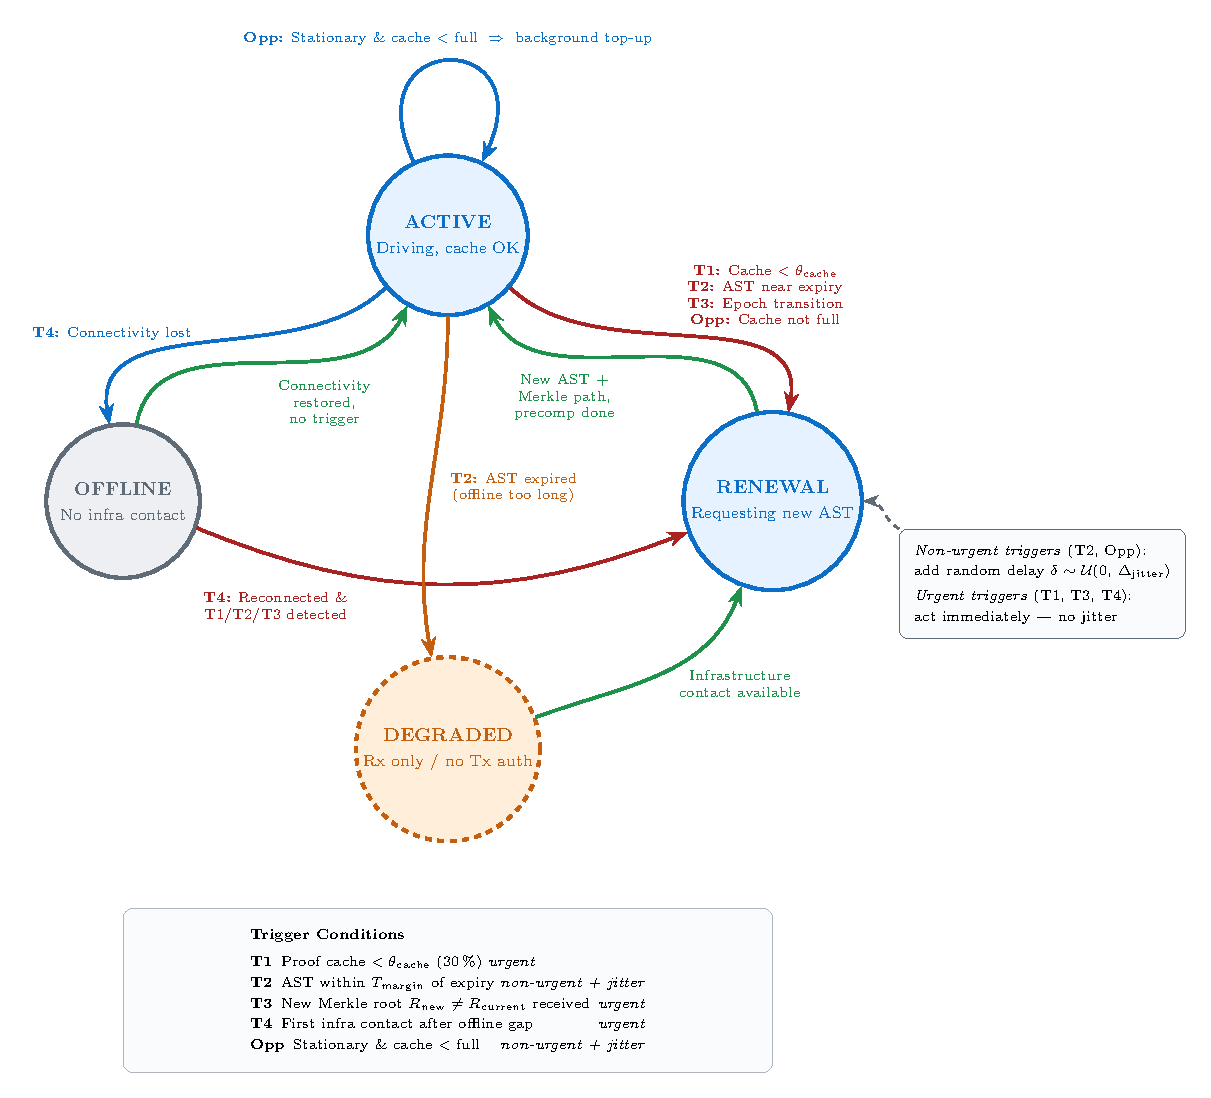
\includegraphics[width=\linewidth]{assets/ast-fsm.pdf}
    \caption{AST request policy finite state machine. States: \textsc{Active}
    (normal driving), \textsc{Offline} (no infrastructure contact), \textsc{Renewal}
    (requesting new AST), \textsc{Degraded} (AST expired, receive-only). Transitions
    are colour-coded: blue = normal flow, red = trigger-fired requests, green =
    recovery transitions, orange = degraded path. Non-urgent triggers (T2, Opp)
    add a random jitter delay $\delta \sim \mathcal{U}(0, \Delta_{\text{jitter}})$
    to prevent timing fingerprinting.}
    \label{fig:ast_fsm}
\end{figure}

\subsection{Epoch Management and Offline Resilience}
\label{sec:epoch}

The Merkle tree of active ASTs is maintained by the AIS and updated at epoch
boundaries. Each update changes the root $R$ and potentially invalidates AST
Merkle paths, creating a challenge for vehicles that are offline during an epoch
transition.

\paragraph{Epoch Duration and Overlap.}
Each AST spans at least two full epochs: $t_{end} - t_{start} \geq 2 \cdot T_{epoch}$.
A vehicle can therefore miss one complete epoch transition without its AST becoming
invalid.

\paragraph{Pre-fetched Merkle Paths for Future Epochs.}
During AST acquisition, the AIS provides the current Merkle path $\pi^{MT}_i$ and
pre-signed commitments for the next epoch root $R_{next}$ (if already computed),
allowing the vehicle to verify proofs against $R_{next}$ without re-contacting the
AIS. This approach is inspired by key chain commitment techniques used in broadcast
authentication protocols for vehicular networks~\cite{muhammad2024}.

\paragraph{Grace Period for Offline Vehicles.}
Verifier vehicles $V_V$ accept proofs referencing the \emph{previous} root $R_{prev}$
for a grace period $T_{grace}$ (e.g., 30 seconds) after each epoch transition.
After $T_{grace}$, only proofs referencing $R_{current}$ are accepted.

\paragraph{Root Dissemination.}
Updated Merkle roots are broadcast by RSUs as part of beacon messages. The root is
small (32 bytes for a Poseidon hash), so dissemination overhead is negligible.

\paragraph{Handling Vehicles Offline at AST Expiry.}
If a vehicle's AST expires while offline, it falls back to \emph{degraded mode}:
it continues to receive and verify messages from other vehicles but does not transmit
authenticated safety messages. The receive-only restriction is a \emph{cryptographic
necessity}: without a valid AST, the vehicle cannot construct a Groth16 proof
satisfying the three conditions of Phase~3, so any transmitted message would be
unconditionally rejected. This behaviour is consistent with IEEE~1609.2/SCMS, where
a vehicle with no valid credential is expected to cease broadcasting~\cite{ieee1609}.

\subsection{ZKP System Selection: Groth16 vs.\ PLONK vs.\ zk-STARK}
\label{sec:zkp_selection}

A natural question is why we select Groth16 rather than PLONK~\cite{gabizon2019plonk}
(which avoids a circuit-specific trusted setup) or zk-STARKs (which require no
trusted setup and offer post-quantum security). Table~\ref{tab:zkp_comparison}
provides a quantitative comparison; we argue that Groth16 is the uniquely
appropriate choice for V2V safety message authentication.

\begin{table}[t]
\centering
\caption{ZKP System Comparison for V2V Safety Message Authentication
(BN254, depth-16 circuit, $\sim$9{,}100 constraints)}
\label{tab:zkp_comparison}
\resizebox{\columnwidth}{!}{%
\begin{tabular}{@{}lccc@{}}
\toprule
\textbf{Property} & \textbf{Groth16} & \textbf{PLONK} & \textbf{zk-STARK} \\
\midrule
Proof size & $\approx$128\,B & $\approx$500--1000\,B & $\approx$50--200\,KB \\
Fits BSM packet ($<$1500\,B) & \checkmark\,(ample) & \checkmark\,(tight) & \texttimes\,(infeasible) \\
Verifier pairings & 3\,(constant) & $\sim$10 + poly evals & Poly-log \\
Prover time (rel.)~\cite{roelink2024,snark_stark_comparison2025} & 1$\times$ & $\sim$2.25--4$\times$ & $\sim$68$\times$ \\
Clean algebraic batch verify & \checkmark & Limited & \texttimes \\
Trusted setup & Circuit-specific & Universal SRS & None \\
Post-quantum & \texttimes & \texttimes & \checkmark \\
\bottomrule
\end{tabular}%
}
\end{table}

\subsubsection{Why Not PLONK?}

PLONK~\cite{gabizon2019plonk} offers a universal SRS and updatable trusted setup,
which are genuine advantages in environments where circuits evolve frequently. For
our application, these advantages do not materialize:

\textbf{Proof size} is the decisive constraint. A PLONK proof comprises 9
$\mathbb{G}_1$ elements plus 7 field elements, totalling 500--1000\,bytes depending
on encoding~\cite{roelink2024}. A Groth16 proof is exactly 128\,bytes. The BSM
payload itself (position, velocity, heading, brake status) occupies
$\approx$200--300\,bytes; a PLONK proof would consume $>$50\% of the remaining
1500-byte packet budget. Groth16's 128\,bytes uses only $\approx$9\% of the budget.

\textbf{Prover speed.} For circuits dominated by Poseidon-based Merkle hashing
(our case), PLONK is $\approx$2.25--4$\times$ slower than Groth16 due to higher
polynomial degree requirements for copy constraints~\cite{roelink2024}.

\textbf{Batch verification.} Groth16's three-point structure
$(A \in \mathbb{G}_1, B \in \mathbb{G}_2, C \in \mathbb{G}_1)$ admits clean
randomised linear combination, reducing $3k$ pairings to $k+3$ via multi-scalar
multiplication. PLONK batch verification requires aggregating multiple polynomial
commitment evaluations and does not achieve the same clean reduction~\cite{lipmaa2024polymath}.

\textbf{Universal SRS is irrelevant.} The V2V authentication circuit is fixed at
firmware deployment time---it encodes fixed operations (Merkle depth $d$, Poseidon
hashing, timestamp range check). A one-time ceremony per circuit version is
acceptable in the vehicular standards context, analogous to IEEE 1609.2's root CA
ceremony.

\subsubsection{Why Not zk-STARKs?}

zk-STARKs are post-quantum secure and require no trusted setup. However, their proof
sizes of 50--200\,KB and prover times $\approx$68$\times$ slower than Groth16 on
equivalent ARM hardware make them completely infeasible for 10\,Hz V2V
broadcasting~\cite{snark_stark_comparison2025}. A single STARK proof would exceed
the entire 802.11p packet size limit by a factor of 30--100.

\subsubsection{Post-Quantum Migration Path}

Groth16 on BN254 does not provide post-quantum security---a legitimate long-term
concern for systems with a 15--20 year deployment lifecycle. This is a known and
accepted tradeoff in current V2X standardization: IEEE 1609.2-2022 also relies on
ECDSA (P-256/P-384) with no post-quantum option. The anticipated migration path is
a firmware-level protocol version update in which the AIS performs a new trusted
setup ceremony for an updated circuit, analogous to CA root key rotation.
Post-quantum zk-SNARKs (lattice-based or hash-based constructions) represent a
natural future extension of this work.

\subsection{Groth16 Trusted Setup: Ceremony and Rationale}
\label{sec:trusted_setup}

Groth16 requires a two-phase structured reference string (SRS) generation:

\begin{itemize}
    \item \textbf{Phase 1 (Powers of Tau, Universal):} A multi-party computation
    (MPC) ceremony generating generic parameters $\{[\tau^i]_{G_1}, [\tau^i]_{G_2}\}$
    up to circuit depth $n$. This phase is circuit-independent. Existing publicly
    verifiable ceremonies (e.g., the Hermez/Polygon perpetual Powers of Tau
    ceremony supporting up to $2^{28}$ constraints) can be directly reused,
    eliminating the need to run Phase~1 from scratch~\cite{snarkjs_github}.

    \item \textbf{Phase 2 (Circuit-Specific):} A second MPC ceremony specialising
    the Phase~1 output to the ULP-V2V-Auth circuit. Participants include automotive
    OEMs, standardisation bodies (IEEE 1609 WG, ETSI ITS), and independent auditors.
    Security holds as long as at least one participant honestly deletes their
    contribution~\cite{bowe2017mpc}. The resulting $(\mathsf{pk}, \mathsf{vk})$ are
    embedded in OBU firmware during manufacturing, analogous to root CA certificates
    in devices today.
\end{itemize}

The trusted setup is a \textbf{one-time, offline} operation performed by the system
deployer. The proving key $\mathsf{pk}$ is pre-loaded into OBU RAM at startup
(avoiding I/O latency during operation). The verification key $\mathsf{vk}$ is
small (a few hundred bytes). Neither requires updating unless the circuit is
redesigned.

\subsection{Concurrent Sender/Receiver Operation}
\label{sec:concurrent}

In highway V2V, a vehicle is simultaneously a \emph{prover} (broadcasting its own
safety messages) and a \emph{verifier} (receiving and authenticating messages from
surrounding vehicles). We propose a \textbf{dual-module architecture}:

\paragraph{Sender Module (SM).}
\begin{itemize}
    \item \emph{Precomputation stage (background):} During AST acquisition and
    whenever CPU slack is available, the SM generates complete proof slots
    committed to predicted BSM content and caches them.
    \item \emph{Online stage (per-message):} At each broadcast interval, the SM
    retrieves the next precomputed slot, binds it to
    $h_m = H_{Poseidon}(m \| t_{current})$, completes the lightweight online proof
    step, and hands $(m, t_{current}, \pi, R)$ to the radio stack.
\end{itemize}

\paragraph{Receiver Module (RM).}
\begin{itemize}
    \item \emph{Collection window:} The RM buffers incoming
    $(m_j, t_j, \pi_j, R_j)$ tuples for a window $T_{window}$ (50--100\,ms).
    \item \emph{Batch verification:} At the end of each window, the RM performs
    batched Groth16 verification. Proofs referencing roots other than $R_{current}$
    (or $R_{prev}$ during $T_{grace}$) are immediately rejected.
    \item \emph{Priority filtering:} Inspired by EABA~\cite{zheng2018eaba}, the RM
    classifies messages by safety priority (e.g., emergency braking $>$ intersection
    warning $>$ routine BSM) and verifies high-priority messages individually and
    immediately, bypassing the batch window.
\end{itemize}

\paragraph{CPU Scheduling.}
The SM and RM run on separate threads (or cores on multi-core OBUs). Precomputation
has background priority; the online proof step and batch verification have real-time
priority. On a single-core OBU, precomputation is interleaved with idle periods
using a cooperative scheduling policy.

\subsection{Precomputation: Circuit-Level Analysis and Tolerability}
\label{sec:precomp_overhead}

Circuit-level analysis of our Circom implementation quantitatively validates the
offline/online decomposition. The constraint breakdown for the depth-16 circuit
($\sim$9{,}100 total) is:

\begin{itemize}
    \item Merkle path (16$\times$ Poseidon-2): $\approx$3{,}872 constraints (42.5\%)
    \item AST leaf hash (Poseidon-5): $\approx$580 constraints (6.4\%)
    \item Timestamp range checks (2$\times$ 32-bit LessEqThan): 64 constraints (0.7\%)
    \item Switcher and wiring: $\approx$4{,}342 constraints (47.7\%)
    \item \textbf{Message hash binding (Poseidon-2): $\approx$242 constraints (2.7\%)}
\end{itemize}

Exactly \textbf{97.3\% of constraints are message-independent}, motivating offline
precomputation of complete Groth16 proofs. The depth-16 circuit strengthens this
decomposition: the message-binding fraction \emph{decreases} from 4.3\% (depth-8)
to 2.7\% as the Merkle path dominates the larger circuit. In the proof-slot cache
model (Section~\ref{sec:bench_cache}), complete proofs are generated offline---each
committed to a predicted BSM content---and stored in a cache. The online step is
then reduced to (i)~dequeuing a pre-generated slot ($< 0.01$\,ms) and (ii)~computing
the Poseidon-2 hash $h_m = H_{\text{Poseidon}}(m \| t_{\text{current}})$ to verify
prediction accuracy ($\mathbf{0.439}$\,ms on RPi~4, directly measured over
5{,}000 runs). The total online cost of 0.439\,ms represents 0.44\% of the 100\,ms
BSM cycle---a $>$8{,}700$\times$ reduction from the full 3{,}841\,ms offline prove
time.

\paragraph{Proof cache sustainability.}
At 10\,Hz broadcasting, one proof slot is consumed per 100\,ms (600 slots/min).
On RPi~4, background precomputation with snarkjs ($\approx$3.84\,s/slot) produces
$\approx$15.6 slots/min, while the native C++ rapidsnark prover reduces this to
$\approx$1{,}422\,ms/slot ($\approx$42.2 slots/min), providing a $2.70\times$
improvement in cache fill rate. With dual-core scheduling, the production rate
($\approx$42/min with rapidsnark) is $14.2\times$ below the consumption rate of
600/min at 10\,Hz. Self-sustaining cache replenishment therefore requires
$14.2\times$ BN254 multi-scalar multiplication (MSM) acceleration over the
RPi~4 baseline---met at the NXP~S32G 25$\times$ acceleration tier or above
(quantified in Section~\ref{sec:experiment}).

For continuous highway operation without intermediate stops, two practical deployment
models address this gap. First, a \textbf{pre-departure fill}: a vehicle pre-generates
sufficient slots for the planned journey during stationary periods (overnight charging,
rest-stop dwell, toll-plaza queue). A 60-minute highway segment at 10\,Hz requires
36{,}000 slots ($\approx$7\,MB of OBU storage), generatable in $\approx$21 minutes
across four CPU cores at the NXP~S32G 10$\times$ tier---well within typical
pre-departure idle time. Second, for vehicles with NXP~S32G 25$\times$ tier or
dedicated ZKP accelerators, cache production exceeds consumption continuously,
requiring no pre-fill.

\paragraph{Hardware acceleration path.}
Automotive-grade processors (NXP S32G, Renesas R-Car H3) include hardware
accelerators for elliptic curve point operations. An important distinction applies:
standard HSE acceleration targets single-point ECDSA operations, while Groth16
proving requires \emph{multi-scalar multiplication} (MSM)---a qualitatively
different workload. At the NXP~S32G 25$\times$ MSM tier, offline prove time drops
to $\approx$57\,ms/slot (self-sustaining); at the 10$\times$ tier ($\approx$142\,ms),
pre-departure fill covers highway trips as described above. Online binding remains
$<$2\,ms regardless of prove speed.

\paragraph{Storage overhead.}
Each precomputed proof slot requires $\approx$2--3 group elements plus the Merkle
path evaluation. For $n=2^{16}$ active ASTs, this is $16 \times 32 = 512$ bytes
per slot; maintaining 16 slots requires $\approx$5--8\,KB of secure storage---well
within OBU capabilities.

\paragraph{Design variant: one-time key binding.}
The position pre-commitment constraint is an artifact of embedding message binding
inside the ZKP circuit via $h_m = H_{\mathit{Poseidon}}(m \| t)$. An alternative
design commits a per-slot \emph{one-time keypair} $(sk^{(s)}_{\mathit{ot}},
pk^{(s)}_{\mathit{ot}})$ inside the proof instead of message content. At broadcast
time, the vehicle signs the actual BSM with $sk^{(s)}_{\mathit{ot}}$ (0.199\,ms
ECDSA-P256 sign), and the receiver verifies both the ZKP proof and the one-time
signature. This eliminates position prediction entirely: proofs are content-agnostic
at generation time and can be used for any BSM---including unpredicted emergency
events---without slot discarding. The tradeoff is $\approx$96 additional bytes per
packet (64\,B one-time signature $+$ 32\,B $pk_{\mathit{ot}}$ in public inputs) and
the need to generate a fresh keypair per slot. We adopt the current Poseidon-binding
design for its smaller packet footprint and simpler circuit; the one-time key variant
is a natural extension for deployments where prediction accuracy is a concern.


% ============================================================
% IV. PROPOSED SYSTEM: ULP-V2V-Auth
% ============================================================
\section{Proposed System: ULP-V2V-Auth}

\subsection{System Model}

The ULP-V2V-Auth system consists of four entity types:

\begin{itemize}
    \item \textbf{Trusted Authority (TA):} A trusted offline entity responsible for
    registering vehicles, issuing long-term anonymous credentials, maintaining the
    Merkle tree of active ASTs, and handling revocation decisions.
    \item \textbf{AST Issuing Service (AIS):} An infrastructure service
    (co-located with RSUs or accessible via cellular networks) that issues
    short-lived Anonymous Session Tokens upon presentation of valid long-term
    credentials. The AIS is authenticated to vehicles via a TA-signed certificate
    (Section~\ref{sec:ast_issuance}).
    \item \textbf{Prover Vehicle ($V_P$):} A vehicle holding a valid AST that
    generates ZKP proofs to authenticate its safety messages, performing offline
    precomputation during AST acquisition and lightweight online proof generation
    per message.
    \item \textbf{Verifier Vehicle ($V_V$):} A receiving vehicle that collects
    incoming safety messages with attached ZKP proofs and performs batch
    verification to authenticate multiple messages simultaneously.
\end{itemize}

The communication model assumes direct V2V sidelink (IEEE 802.11p/802.11bd or
C-V2X Mode~4) for safety message exchange, and intermittent infrastructure access
(RSU, cellular, or Wi-Fi) for AST acquisition and Merkle root updates.

\begin{figure}[t]
    \centering
    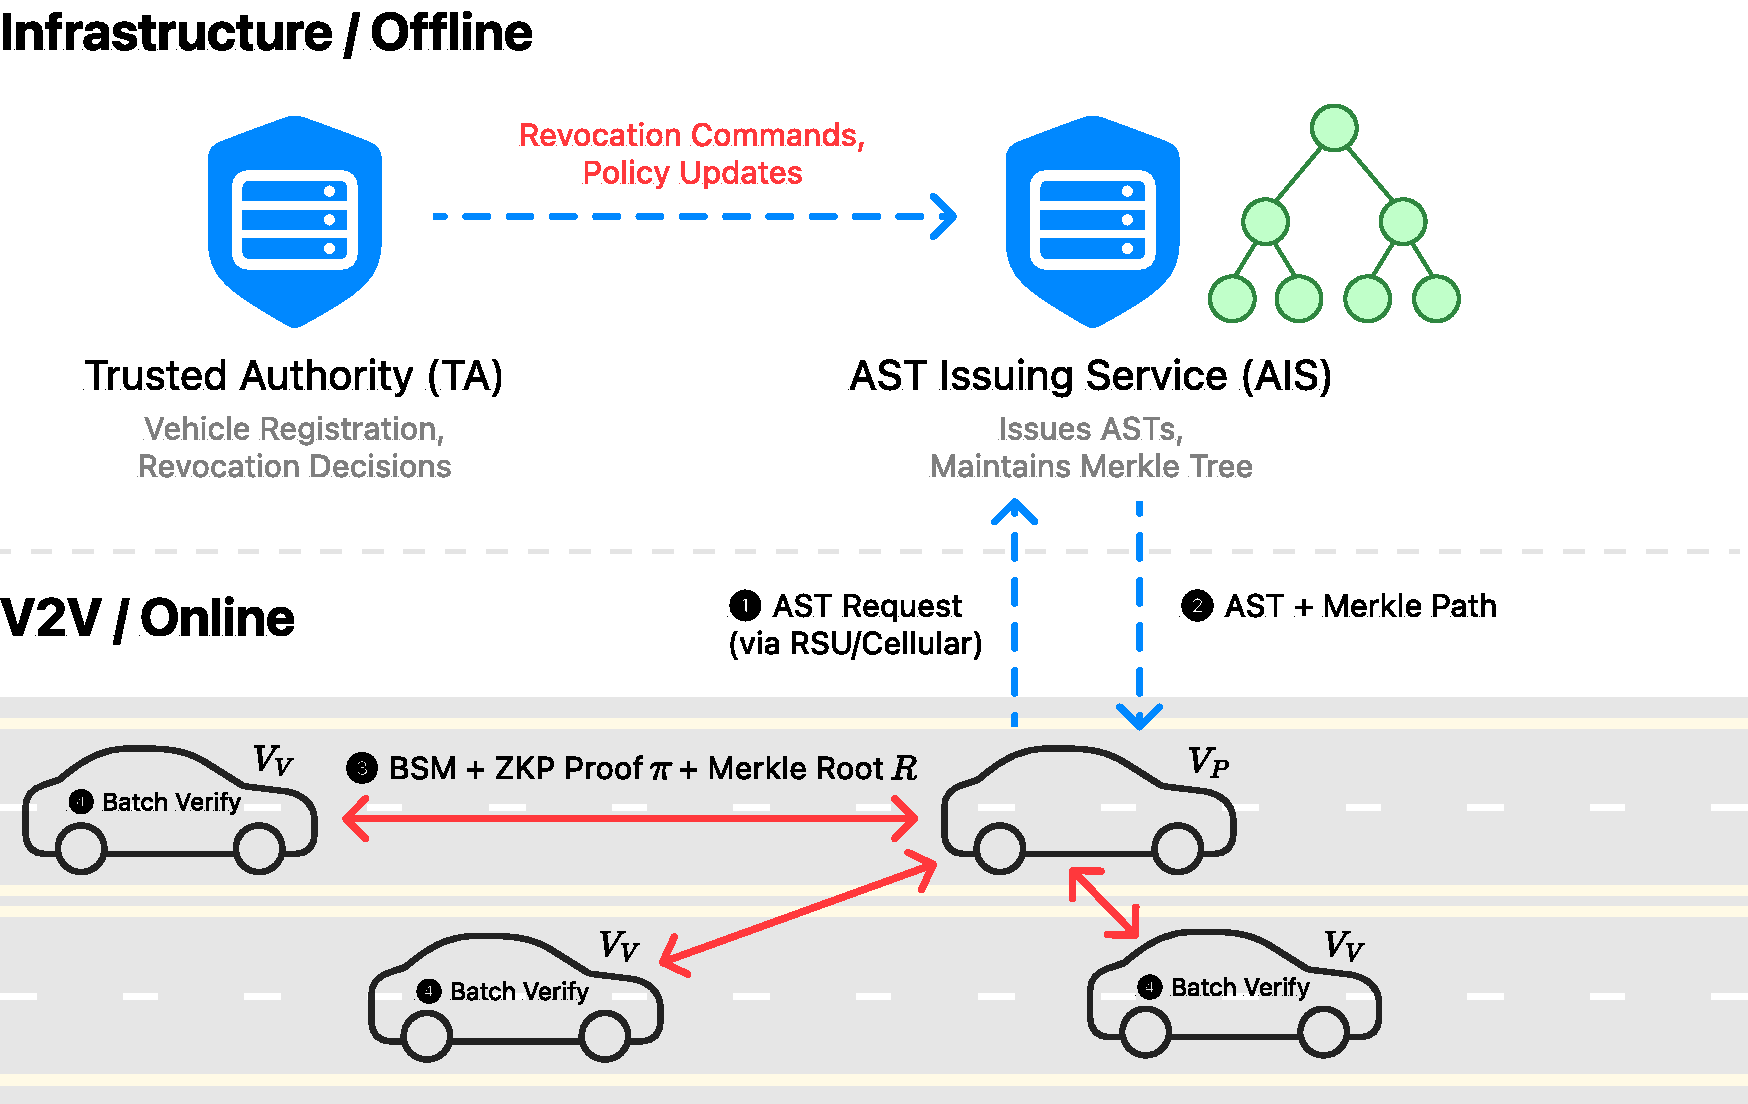
\includegraphics[width=\linewidth]{assets/system_model.pdf}
    \caption{System model of ULP-V2V-Auth showing the four entities and their
    interactions across offline (AST acquisition) and online (V2V authentication)
    phases.}
    \label{fig:system_model}
\end{figure}

\subsection{Cryptographic Preliminaries}

\subsubsection{Bilinear Pairing}
Let $\mathbb{G}_1$, $\mathbb{G}_2$, and $\mathbb{G}_T$ be cyclic groups of prime
order $p$. A bilinear pairing is a map $e: \mathbb{G}_1 \times \mathbb{G}_2
\rightarrow \mathbb{G}_T$ satisfying bilinearity ($e(aP, bQ) = e(P, Q)^{ab}$),
non-degeneracy, and efficient computability. We use the BN254 elliptic curve,
providing approximately 128-bit security and efficient pairing computation.

\subsubsection{Groth16 zk-SNARK}
Groth16~\cite{groth2016} is a pairing-based zk-SNARK producing proofs of only three
group elements $(A \in \mathbb{G}_1, B \in \mathbb{G}_2, C \in \mathbb{G}_1)$,
yielding a proof size of $\approx$128 bytes on BN254. Verification requires exactly
3 pairing operations and is constant-time regardless of circuit size. The system
consists of three algorithms: $\mathsf{Setup}(\mathcal{C}) \rightarrow (\mathsf{pk},
\mathsf{vk})$; $\mathsf{Prove}(\mathsf{pk}, x, w) \rightarrow \pi$; and
$\mathsf{Verify}(\mathsf{vk}, x, \pi) \rightarrow \{0, 1\}$.

\subsubsection{Merkle Hash Tree}
A Merkle hash tree is a binary tree where each leaf contains the hash of a data block
and each internal node contains the hash of its two children. A membership proof
(Merkle path) for a tree with $n$ leaves consists of $\lceil \log_2 n \rceil$ hash
values. We use the Poseidon hash function~\cite{poseidon2021}, optimized for
arithmetic circuits (SNARK-friendly), requiring significantly fewer constraints
than SHA-256 when embedded in a ZKP circuit.

\subsection{Protocol Design}

The ULP-V2V-Auth protocol operates in four phases, as illustrated in
Fig.~\ref{fig:protocol_flow}.

\begin{figure}[t]
    \centering
    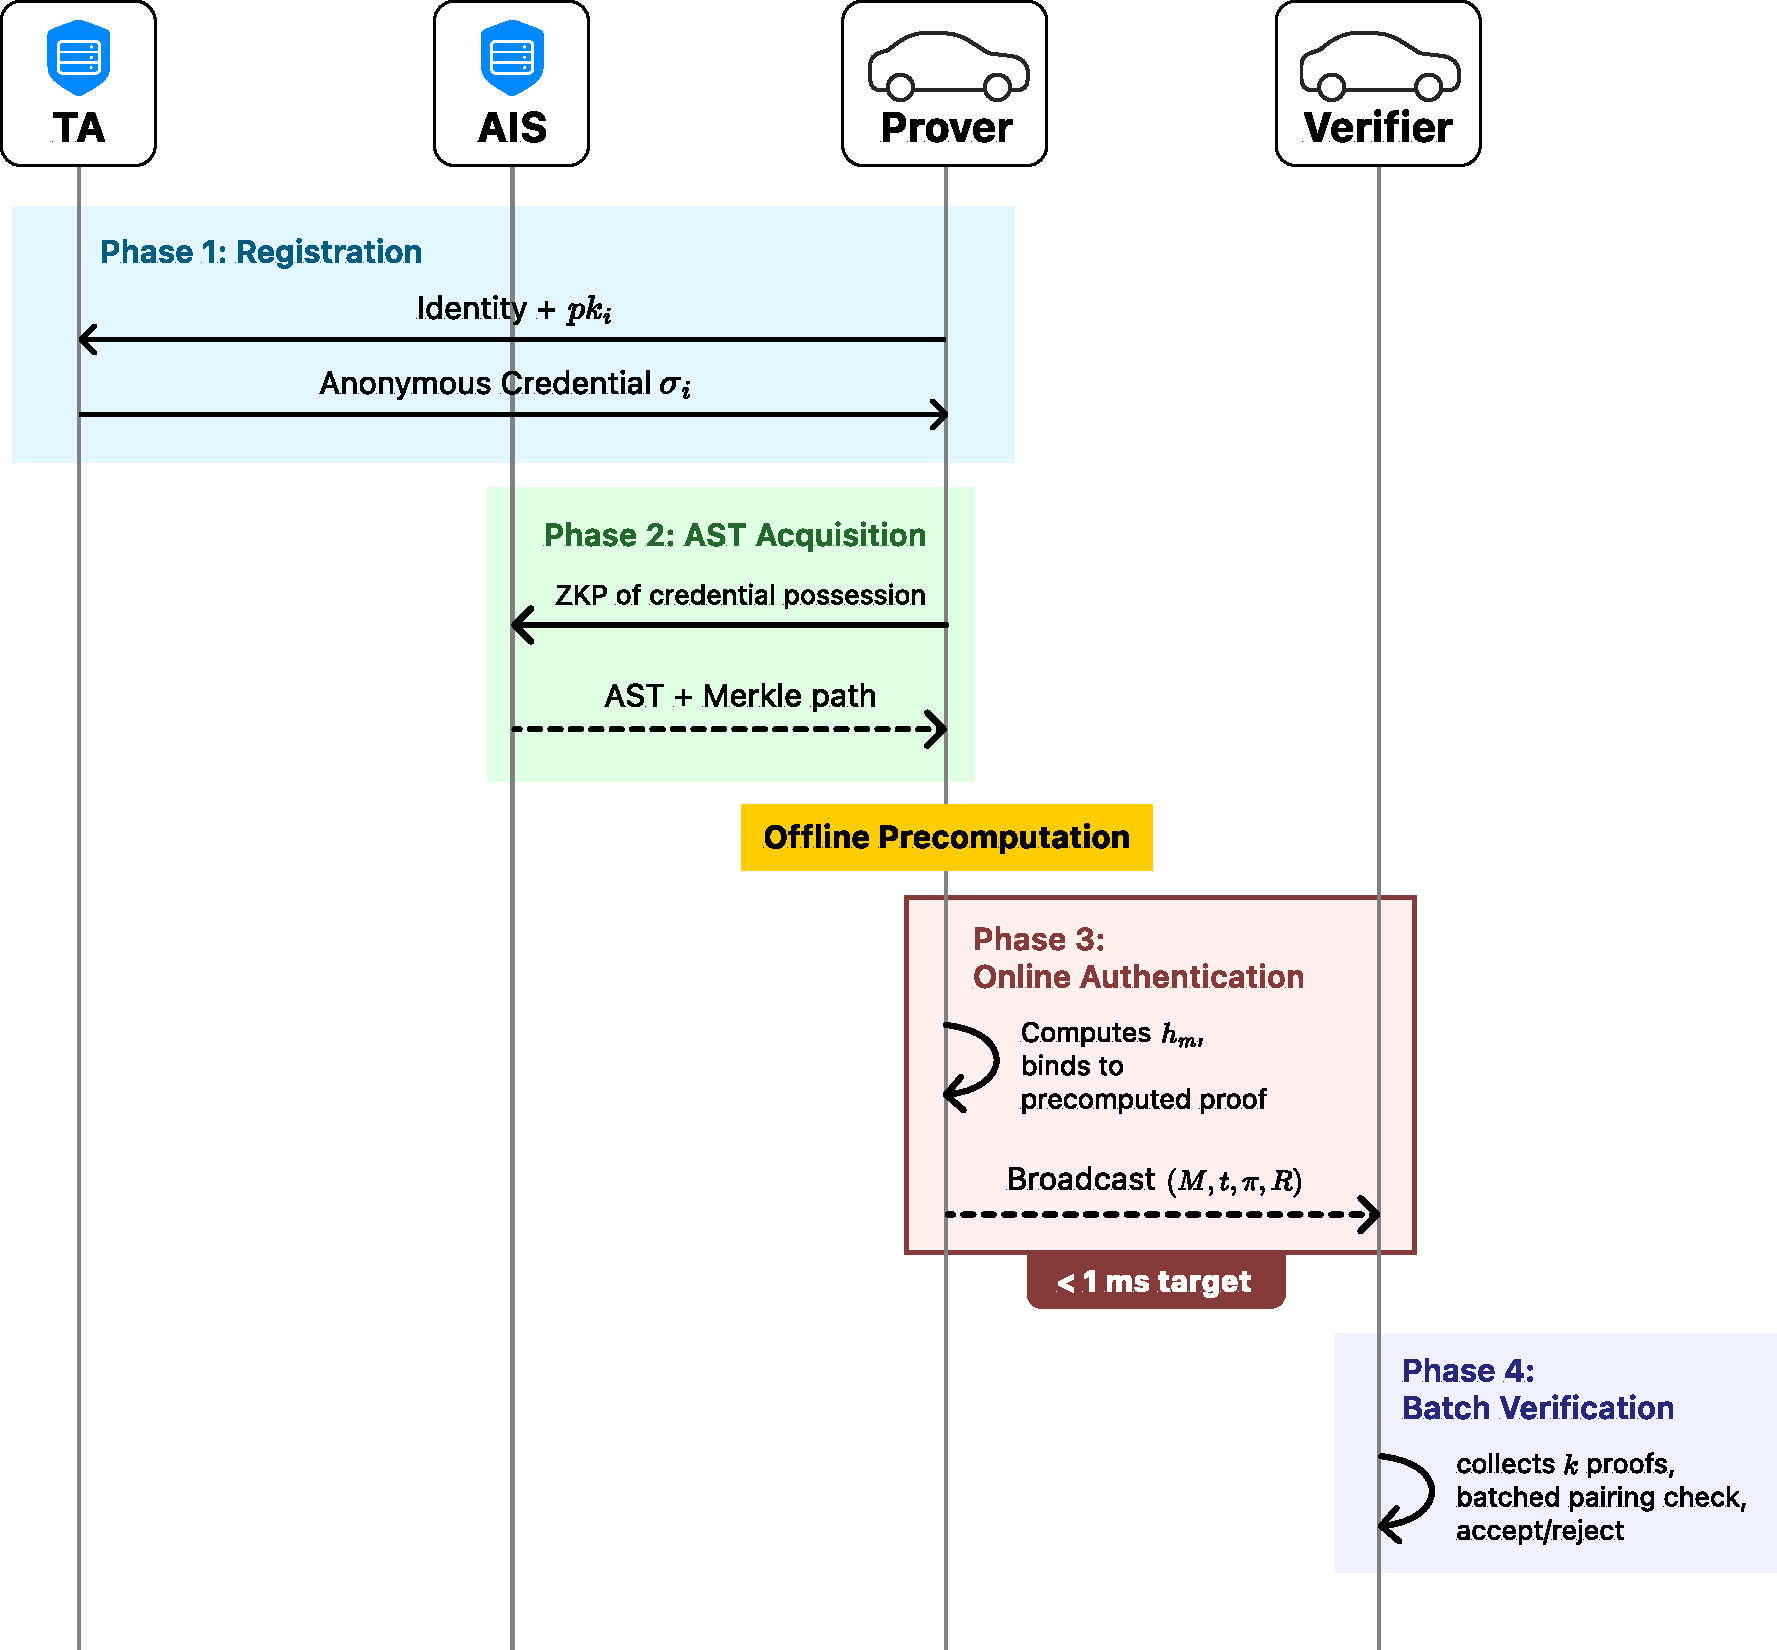
\includegraphics[width=\linewidth]{assets/seqdia.pdf}
    \caption{Protocol flow of ULP-V2V-Auth showing the four phases: (1) Registration,
    (2) AST Acquisition, (3) Online Authentication, and (4) Batch Verification.}
    \label{fig:protocol_flow}
\end{figure}

\subsubsection{Phase 1: Vehicle Registration (One-Time)}
A vehicle $V_i$ registers with the TA through a secure out-of-band channel (Fig.~\ref{fig:phase1}):
\begin{enumerate}
    \item $V_i$ generates a long-term key pair $(sk_i, pk_i)$ on the BN254 curve.
    \item $V_i$ presents its real-world identity (e.g., VIN) and $pk_i$ to the TA.
    \item The TA verifies the vehicle's legitimacy and issues an anonymous credential
    $\sigma_i = \mathsf{Sign}_{sk_{TA}}(H(pk_i \| \mathsf{nonce}))$ via blind
    signature, attesting to $V_i$'s legitimacy without being linkable to $V_i$'s
    real identity by any party other than the TA.
    \item $V_i$ stores $(sk_i, \sigma_i, pk_{TA})$ securely in its OBU's
    tamper-proof module.
\end{enumerate}

\begin{figure}[t]
    \centering
    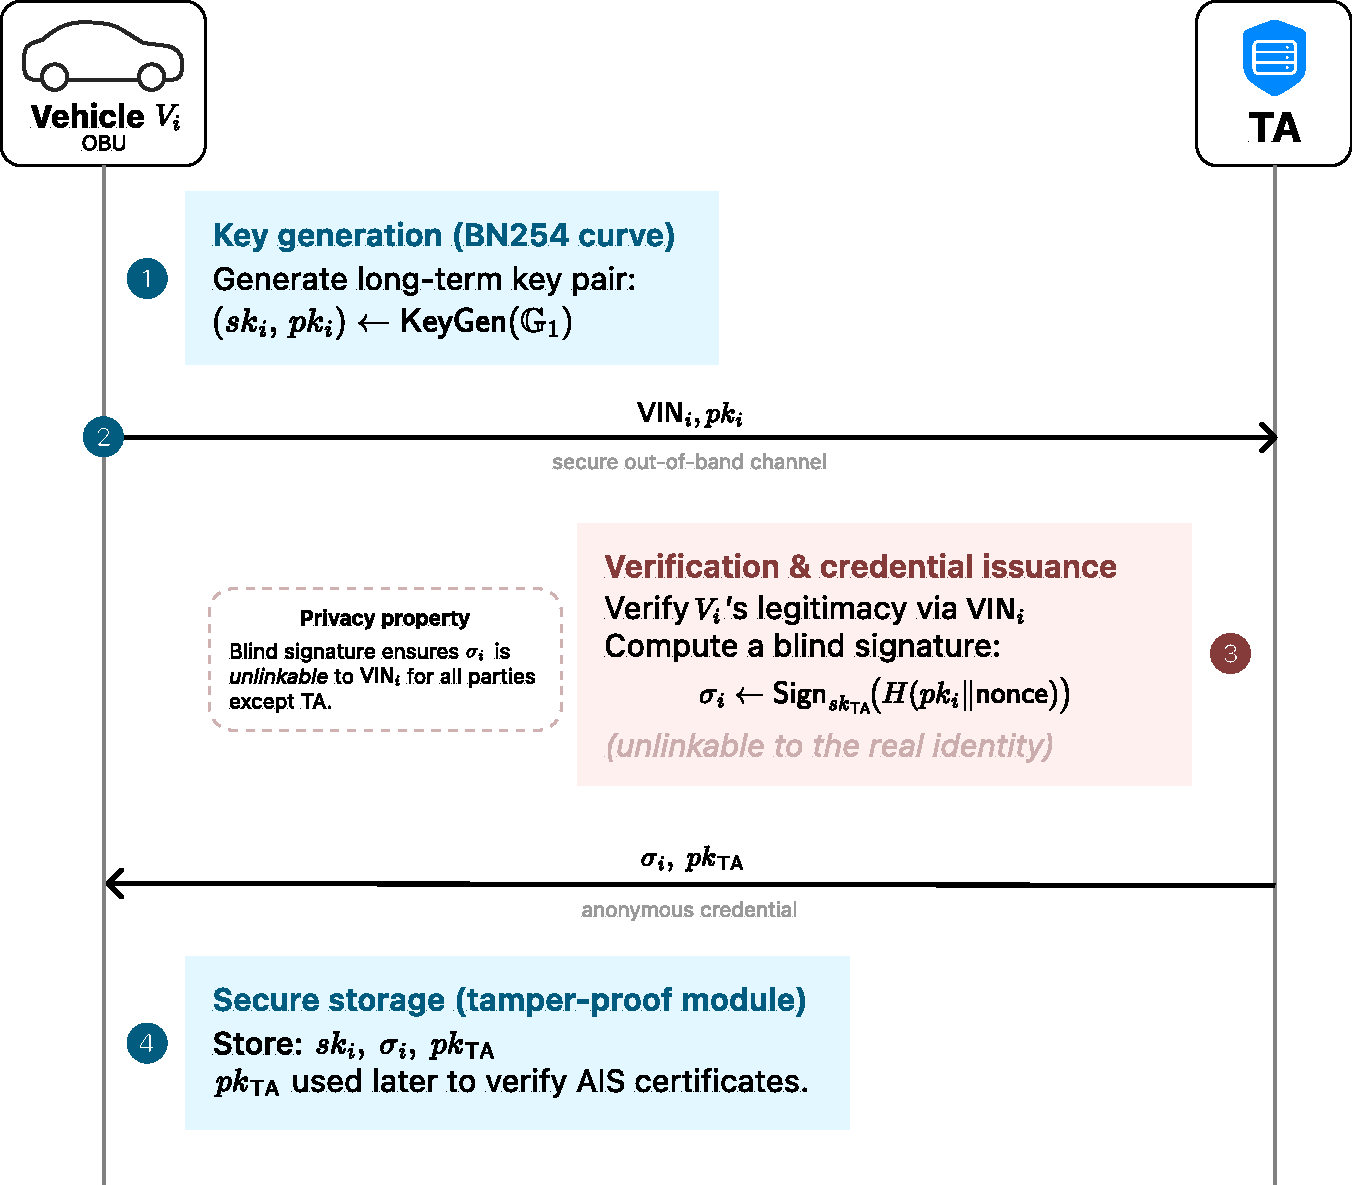
\includegraphics[width=\linewidth]{assets/phase1.pdf}
    \caption{Phase 1: Vehicle registration. $V_i$ submits $pk_i$ to the Trusted
    Authority, which issues an anonymous credential $\sigma_i$ via blind signature.
    The TA's public key $pk_{TA}$ is pre-loaded into the OBU for subsequent AIS
    certificate verification.}
    \label{fig:phase1}
\end{figure}

\begin{algorithm}[t]
\caption{Vehicle Registration --- Phase 1 (One-Time)}
\label{alg:registration}
\begin{algorithmic}[1]
\REQUIRE Vehicle identity $\mathsf{VIN}$, BN254 curve parameters, TA public key $pk_{TA}$
\ENSURE $(sk_i, pk_i, \sigma_i, pk_{TA})$ stored in OBU tamper-proof module
\STATE $(sk_i, pk_i) \leftarrow \mathsf{KeyGen}(\mathsf{BN254})$
\STATE Send $(\mathsf{VIN},\; pk_i)$ to TA over secure out-of-band channel
\STATE \textbf{[TA side]} Verify $\mathsf{VIN}$ legitimacy; abort if invalid
\STATE \textbf{[TA side]} $\mathsf{nonce} \xleftarrow{\$} \{0,1\}^{256}$
\STATE \textbf{[TA side]} $\sigma_i \leftarrow \mathsf{Sign}_{sk_{TA}}\!\bigl(H(pk_i \;\|\; \mathsf{nonce})\bigr)$
\STATE \textbf{[TA side]} Transmit $\sigma_i$ to $V_i$ over secure channel
\STATE $V_i$ verifies $\sigma_i$ against $pk_{TA}$; abort if invalid
\STATE Store $(sk_i,\; \sigma_i,\; pk_{TA})$ in OBU tamper-proof module
\end{algorithmic}
\end{algorithm}

\subsubsection{Phase 2: AST Acquisition (Periodic, Offline)}
When $V_i$ has infrastructure access, it requests a fresh AST per
Section~\ref{sec:ast_policy} (Fig.~\ref{fig:phase2}):
\begin{enumerate}
    \item $V_i$ connects to the AIS and verifies $\mathsf{cert}_{AIS}$ against
    $pk_{TA}$. If verification fails, the session is aborted.
    \item $V_i$ presents a ZKP of possession of valid credential $\sigma_i$,
    without revealing $\sigma_i$ or $pk_i$.
    \item The AIS generates an AST:
    $\mathsf{AST}_i = \{sid_i,\ t_{start},\ t_{end},\ cap_i,\ r_i\}$,
    where $sid_i$ is a random session identifier, $[t_{start}, t_{end}]$ spans at
    least two epochs, $cap_i$ encodes vehicle capabilities, and $r_i$ is a random
    blinding factor.
    \item The AIS computes
    $\mathsf{leaf}_i = H_{Poseidon}(sid_i \| t_{start} \| t_{end} \| cap_i \| r_i)$,
    inserts it into the Merkle tree, and returns $(R_{new}, \pi^{MT}_i,
    \mathsf{sig}_{AIS}, R_{next})$ to $V_i$, all signed as
    $\mathsf{sig}_{AIS} = \mathsf{Sign}_{sk_{AIS}}(H(R_{new} \| \pi^{MT}_i))$.
    \item \textbf{Offline Precomputation (Proof-Slot Cache):} $V_i$ precomputes
    $N_{cache}$ \emph{complete} Groth16 proofs, each committed to a predicted BSM
    content $(m^{(s)}_{\mathit{pred}}, t^{(s)}_{\mathit{pred}})$ for the next
    driving segment. Each slot stores the complete proof $\pi^{(s)}$ and its public
    inputs $(R,\; t^{(s)}_{\mathit{pred}},\; h^{(s)}_{m})$ where
    $h^{(s)}_{m} = H_{\mathit{Poseidon}}(m^{(s)}_{\mathit{pred}} \|
    t^{(s)}_{\mathit{pred}})$. The 97.3\% of circuit constraints that are
    message-independent (Merkle path, AST fields, timestamp range) make
    offline precomputation the dominant cost; only the per-slot message commitment
    varies between slots.
\end{enumerate}

\begin{figure}[t]
    \centering
    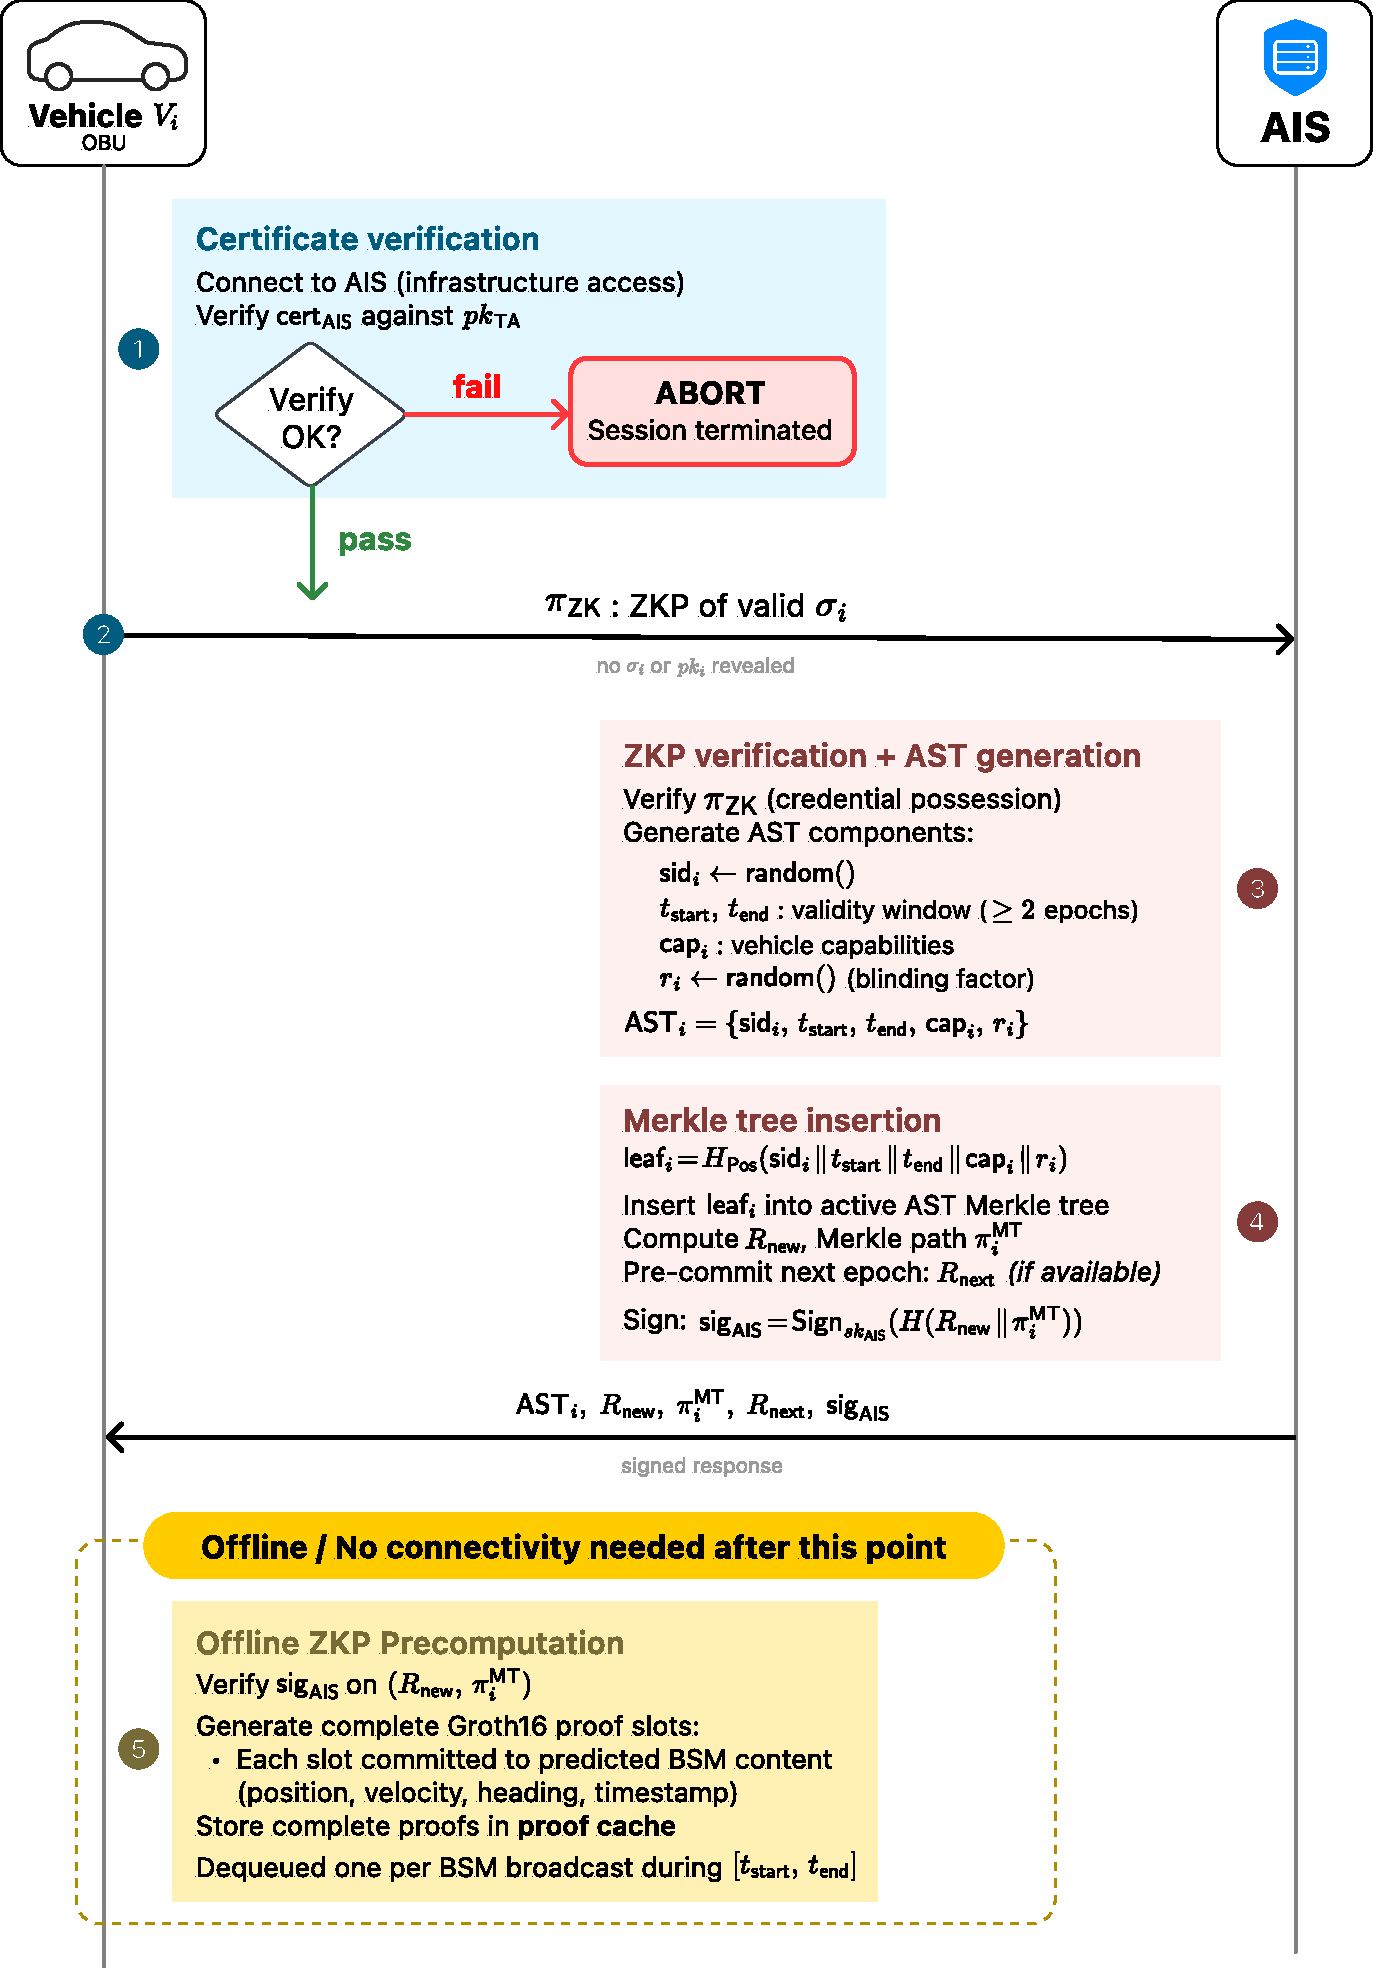
\includegraphics[width=\linewidth]{assets/phase2.pdf}
    \caption{Phase 2: AST acquisition. $V_i$ verifies the AIS certificate, presents
    a ZKP of credential possession, and receives an AST with Merkle path
    $\pi^{MT}_i$. Complete Groth16 proof slots are precomputed offline and stored
    in the proof-slot cache before the next driving segment.}
    \label{fig:phase2}
\end{figure}

\begin{algorithm}[t]
\caption{AST Acquisition and Offline Precomputation --- Phase 2 (Periodic)}
\label{alg:ast_acquisition}
\begin{algorithmic}[1]
\REQUIRE $(sk_i, \sigma_i, pk_{TA})$, proving key $\mathsf{pk}$, cache capacity $N_{\mathit{cache}}$
\ENSURE Proof cache $\mathcal{C}$ filled with $N_{\mathit{cache}}$ complete proof slots; current root $R$ stored
\STATE Connect to AIS via available infrastructure (RSU / cellular / Wi-Fi)
\STATE Retrieve $\mathsf{cert}_{AIS} = (pk_{AIS},\; \mathsf{validity},\; \mathsf{sig}_{TA})$ from AIS
\IF{$\mathsf{Verify}_{pk_{TA}}(\mathsf{cert}_{AIS}) = 0$}
    \STATE \textbf{abort} and report incident to TA
\ENDIF
\STATE $\pi_{\sigma} \leftarrow \mathsf{Prove}(\mathsf{pk},\; \emptyset,\; \sigma_i)$
    \hfill \COMMENT{ZKP of credential possession}
\STATE Send $\pi_{\sigma}$ to AIS; AIS verifies and issues $\mathsf{AST}_i$
\STATE \quad $\mathsf{leaf}_i \leftarrow H_{\mathit{Poseidon}}(sid_i \;\|\; t_{\mathit{start}} \;\|\; t_{\mathit{end}} \;\|\; \mathit{cap}_i \;\|\; r_i)$
\STATE Receive $(R_{\mathit{new}},\; \pi^{MT}_i,\; \mathsf{sig}_{AIS},\; R_{\mathit{next}})$ from AIS
\IF{$\mathsf{Verify}_{pk_{AIS}}\!\bigl(\mathsf{sig}_{AIS},\; H(R_{\mathit{new}} \;\|\; \pi^{MT}_i)\bigr) = 0$}
    \STATE \textbf{abort}
\ENDIF
\STATE Store $(\mathsf{AST}_i,\; \pi^{MT}_i,\; R_{\mathit{new}},\; R_{\mathit{next}})$ in OBU secure storage
\FOR{$s \leftarrow 1$ \TO $N_{\mathit{cache}}$}
    \STATE $(m^{(s)}_{\mathit{pred}},\; t^{(s)}_{\mathit{pred}}) \leftarrow \mathsf{PredictBSM}(s)$
        \hfill \COMMENT{GPS/IMU-based trajectory prediction}
    \STATE $h^{(s)}_m \leftarrow H_{\mathit{Poseidon}}(m^{(s)}_{\mathit{pred}} \| t^{(s)}_{\mathit{pred}})$
    \STATE $\pi^{(s)} \leftarrow \mathsf{Groth16.Prove}(\mathsf{pk},\; (R_{\mathit{new}},\; t^{(s)}_{\mathit{pred}},\; h^{(s)}_m),\; (\mathsf{AST}_i,\; \pi^{MT}_i,\; m^{(s)}_{\mathit{pred}}))$
    \STATE Append $(\pi^{(s)},\; h^{(s)}_m,\; t^{(s)}_{\mathit{pred}})$ to proof cache $\mathcal{C}$
\ENDFOR
\STATE Mark all slots in $\mathcal{C}$ as bound to root $R_{\mathit{new}}$
\end{algorithmic}
\end{algorithm}

\subsubsection{Phase 3: Online V2V Authentication (Per Message)}
When $V_i$ broadcasts safety message $m$ at time $t_{\mathit{cur}}$
(Fig.~\ref{fig:phase3}):
\begin{enumerate}
    \item $V_i$ dequeues the next proof slot $(\pi^{(s)}, h^{(s)}_m,
    t^{(s)}_{\mathit{pred}})$ from its cache. This operation is $< 0.01$\,ms.
    \item $V_i$ computes $h_m = H_{\mathit{Poseidon}}(m \| t_{\mathit{cur}})$ to
    verify prediction accuracy. If $h_m \neq h^{(s)}_m$ (i.e., the actual BSM
    content deviates beyond GPS tolerance from the pre-committed content), the slot
    is discarded and the next slot is tried; otherwise the slot is valid.
    \item The pre-generated proof $\pi^{(s)}$ already proves:
    \begin{equation}
    \begin{aligned}
        \text{``I know } & \mathsf{AST}_i \text{ and } \pi^{MT}_i \text{ such that:} \\
        & (1)\ \mathsf{Verify}_{MT}(\pi^{MT}_i, \mathsf{leaf}_i, R) = 1 \\
        & (2)\ t_{start} \leq t_{\mathit{pred}} \leq t_{end} \\
        & (3)\ h^{(s)}_m = H_{Poseidon}(m^{(s)}_{\mathit{pred}} \| t^{(s)}_{\mathit{pred}}) \text{''}
    \end{aligned}
    \end{equation}
    Public inputs: $(R,\; t^{(s)}_{\mathit{pred}},\; h^{(s)}_m)$. No proof
    computation occurs online.
    \item $V_i$ broadcasts $(m,\ t_{\mathit{cur}},\ \pi^{(s)},\ R)$. The verifier
    independently recomputes $H_{\mathit{Poseidon}}(m \| t_{\mathit{cur}})$ and
    checks it against $h^{(s)}_m$ in the proof's public inputs.
\end{enumerate}

The entire online phase is dominated by step~(2): one Poseidon-2 hash evaluation
(0.437\,ms, directly measured). No elliptic curve operations occur online---the
proof is already complete. Position prediction accuracy of $<3$\,m at highway
speeds (see Section~\ref{sec:bench_cache}) ensures slots are consumed without
discarding under normal driving.

\begin{figure}[t]
    \centering
    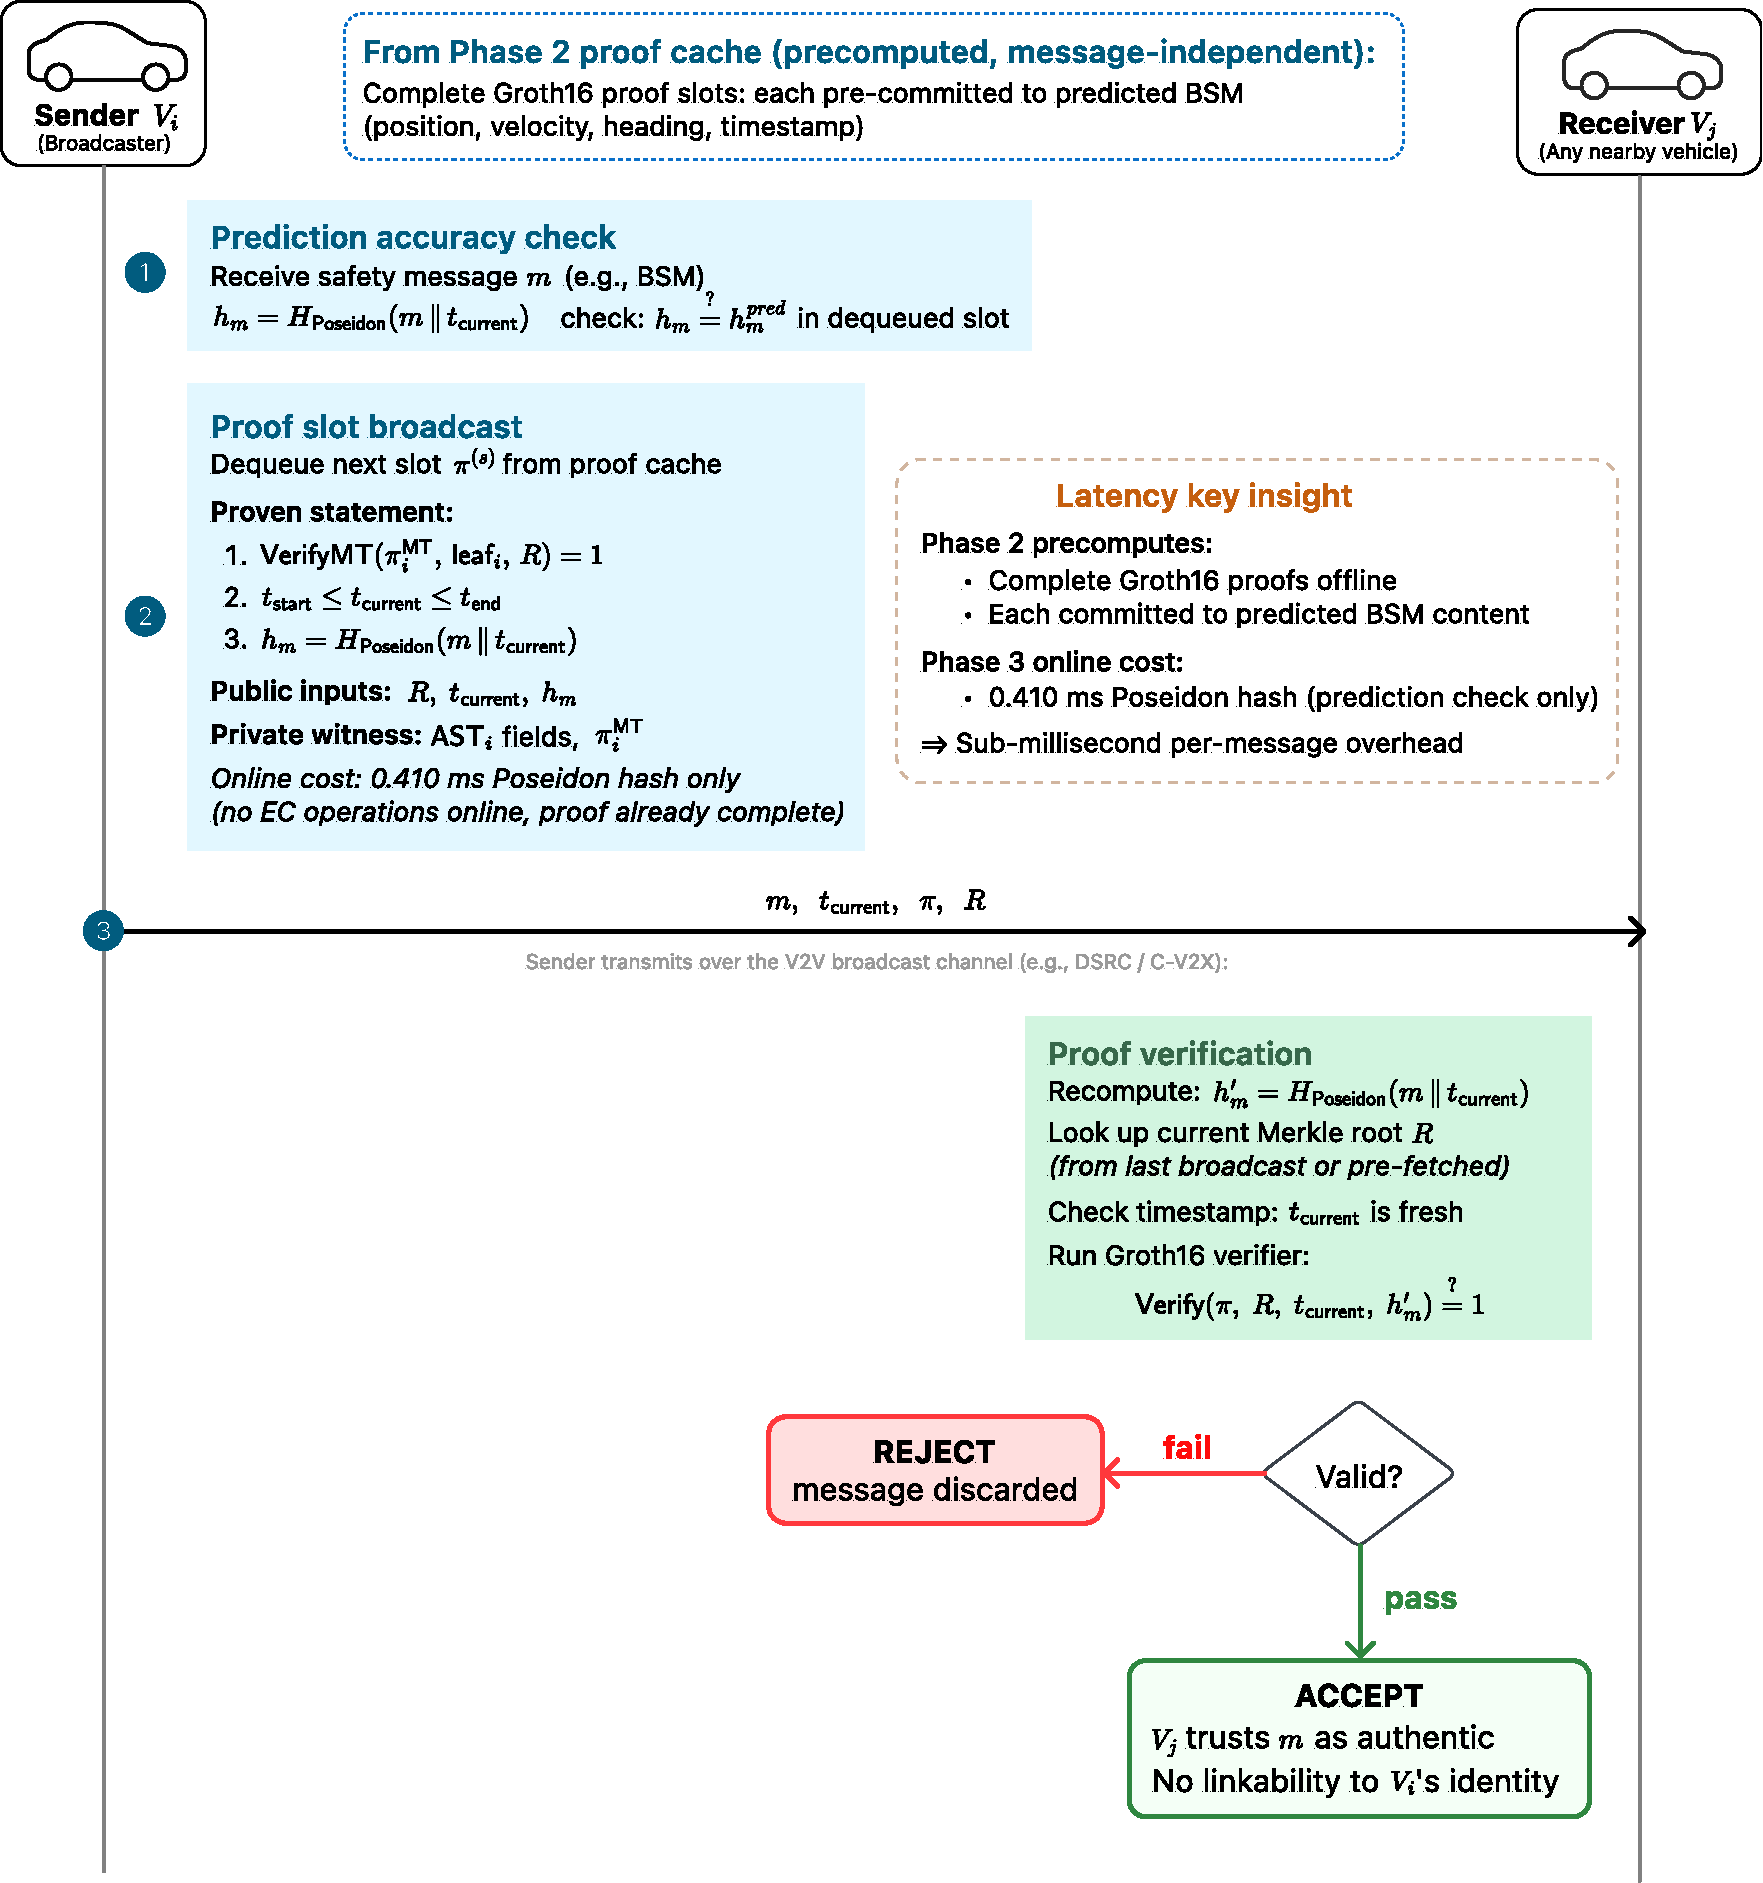
\includegraphics[width=\linewidth]{assets/phase3.pdf}
    \caption{Phase 3: Online V2V authentication. $V_P$ dequeues a pre-generated
    proof slot and computes $h_m = H_{\text{Poseidon}}(m \| t_{\text{current}})$
    to confirm prediction accuracy. No elliptic curve operations occur online. The
    tuple $(m, t_{\text{current}}, \pi, R)$ is broadcast over the V2V channel with
    total online cost 0.439\,ms.}
    \label{fig:phase3}
\end{figure}

\begin{algorithm}[t]
\caption{Online Proof Broadcast (Phase 3)}
\label{alg:online_proof}
\begin{algorithmic}[1]
\REQUIRE Proof cache $\mathcal{C} = \{(\pi^{(s)}, h^{(s)}_m, t^{(s)}_{\mathit{pred}})\}$, message $m$, timestamp $t_{\mathit{cur}}$
\ENSURE Broadcast authenticated BSM or discard slot
\STATE Dequeue next slot $(\pi^{(s)}, h^{(s)}_m, t^{(s)}_{\mathit{pred}})$ from $\mathcal{C}$
    \hfill \COMMENT{$< 0.01$\,ms}
\STATE $h_m \leftarrow H_{\mathrm{Poseidon}}(m \| t_{\mathit{cur}})$
    \hfill \COMMENT{$0.437$\,ms, irreducible online cost}
\IF{$h_m \neq h^{(s)}_m$}
    \STATE Discard slot; try next slot \hfill \COMMENT{prediction miss; rare at highway speeds}
\ENDIF
\STATE Broadcast $(m,\; t_{\mathit{cur}},\; \pi^{(s)},\; R)$
    \hfill \COMMENT{proof already complete; no EC ops online}
\end{algorithmic}
\end{algorithm}

\subsubsection{Phase 4: Batch Verification (Receiver Side)}
Verifier vehicle $V_V$ receiving multiple authenticated messages (Fig.~\ref{fig:phase4}):
\begin{enumerate}
    \item $V_V$ checks that the Merkle root $R$ in each message matches
    $R_{current}$ (or $R_{prev}$ during $T_{grace}$). Messages with unrecognised
    roots are immediately discarded.
    \item $V_V$ applies priority filtering: emergency-class messages are
    individually verified immediately; standard BSMs are buffered for batch
    verification.
    \item $V_V$ collects $k$ standard proofs within window $T_{window}$
    (50--100\,ms).
    \item $V_V$ performs batched Groth16 verification. For individual verification:
    \begin{equation}
        e(A_j, B_j) = e(\alpha, \beta) \cdot e(L_j, \gamma) \cdot e(C_j, \delta)
    \end{equation}
    For batch verification of $k$ proofs, the verifier samples random scalars
    $\rho_1, \ldots, \rho_k$ and checks:
    \begin{equation}
        \prod_{j=1}^{k} e(A_j, B_j)^{\rho_j} = e(\alpha, \beta)^{\sum \rho_j}
        \cdot \prod_{j=1}^{k} e(L_j, \gamma)^{\rho_j}
        \cdot \prod_{j=1}^{k} e(C_j, \delta)^{\rho_j}
    \end{equation}
    Using multi-scalar multiplication, this reduces pairings from $3k$
    (individual) to $k+3$ (batched).
    \item If batch verification fails, $V_V$ applies the Divide-and-Conquer
    Verifier (DCV, Algorithm~\ref{alg:dcv_fallback}) to identify invalid
    proof(s) in $O(w \log k)$ sub-batch operations rather than $O(k)$ individual
    verifications, where $w$ is the number of invalid proofs.
\end{enumerate}

\begin{figure}[t]
    \centering
    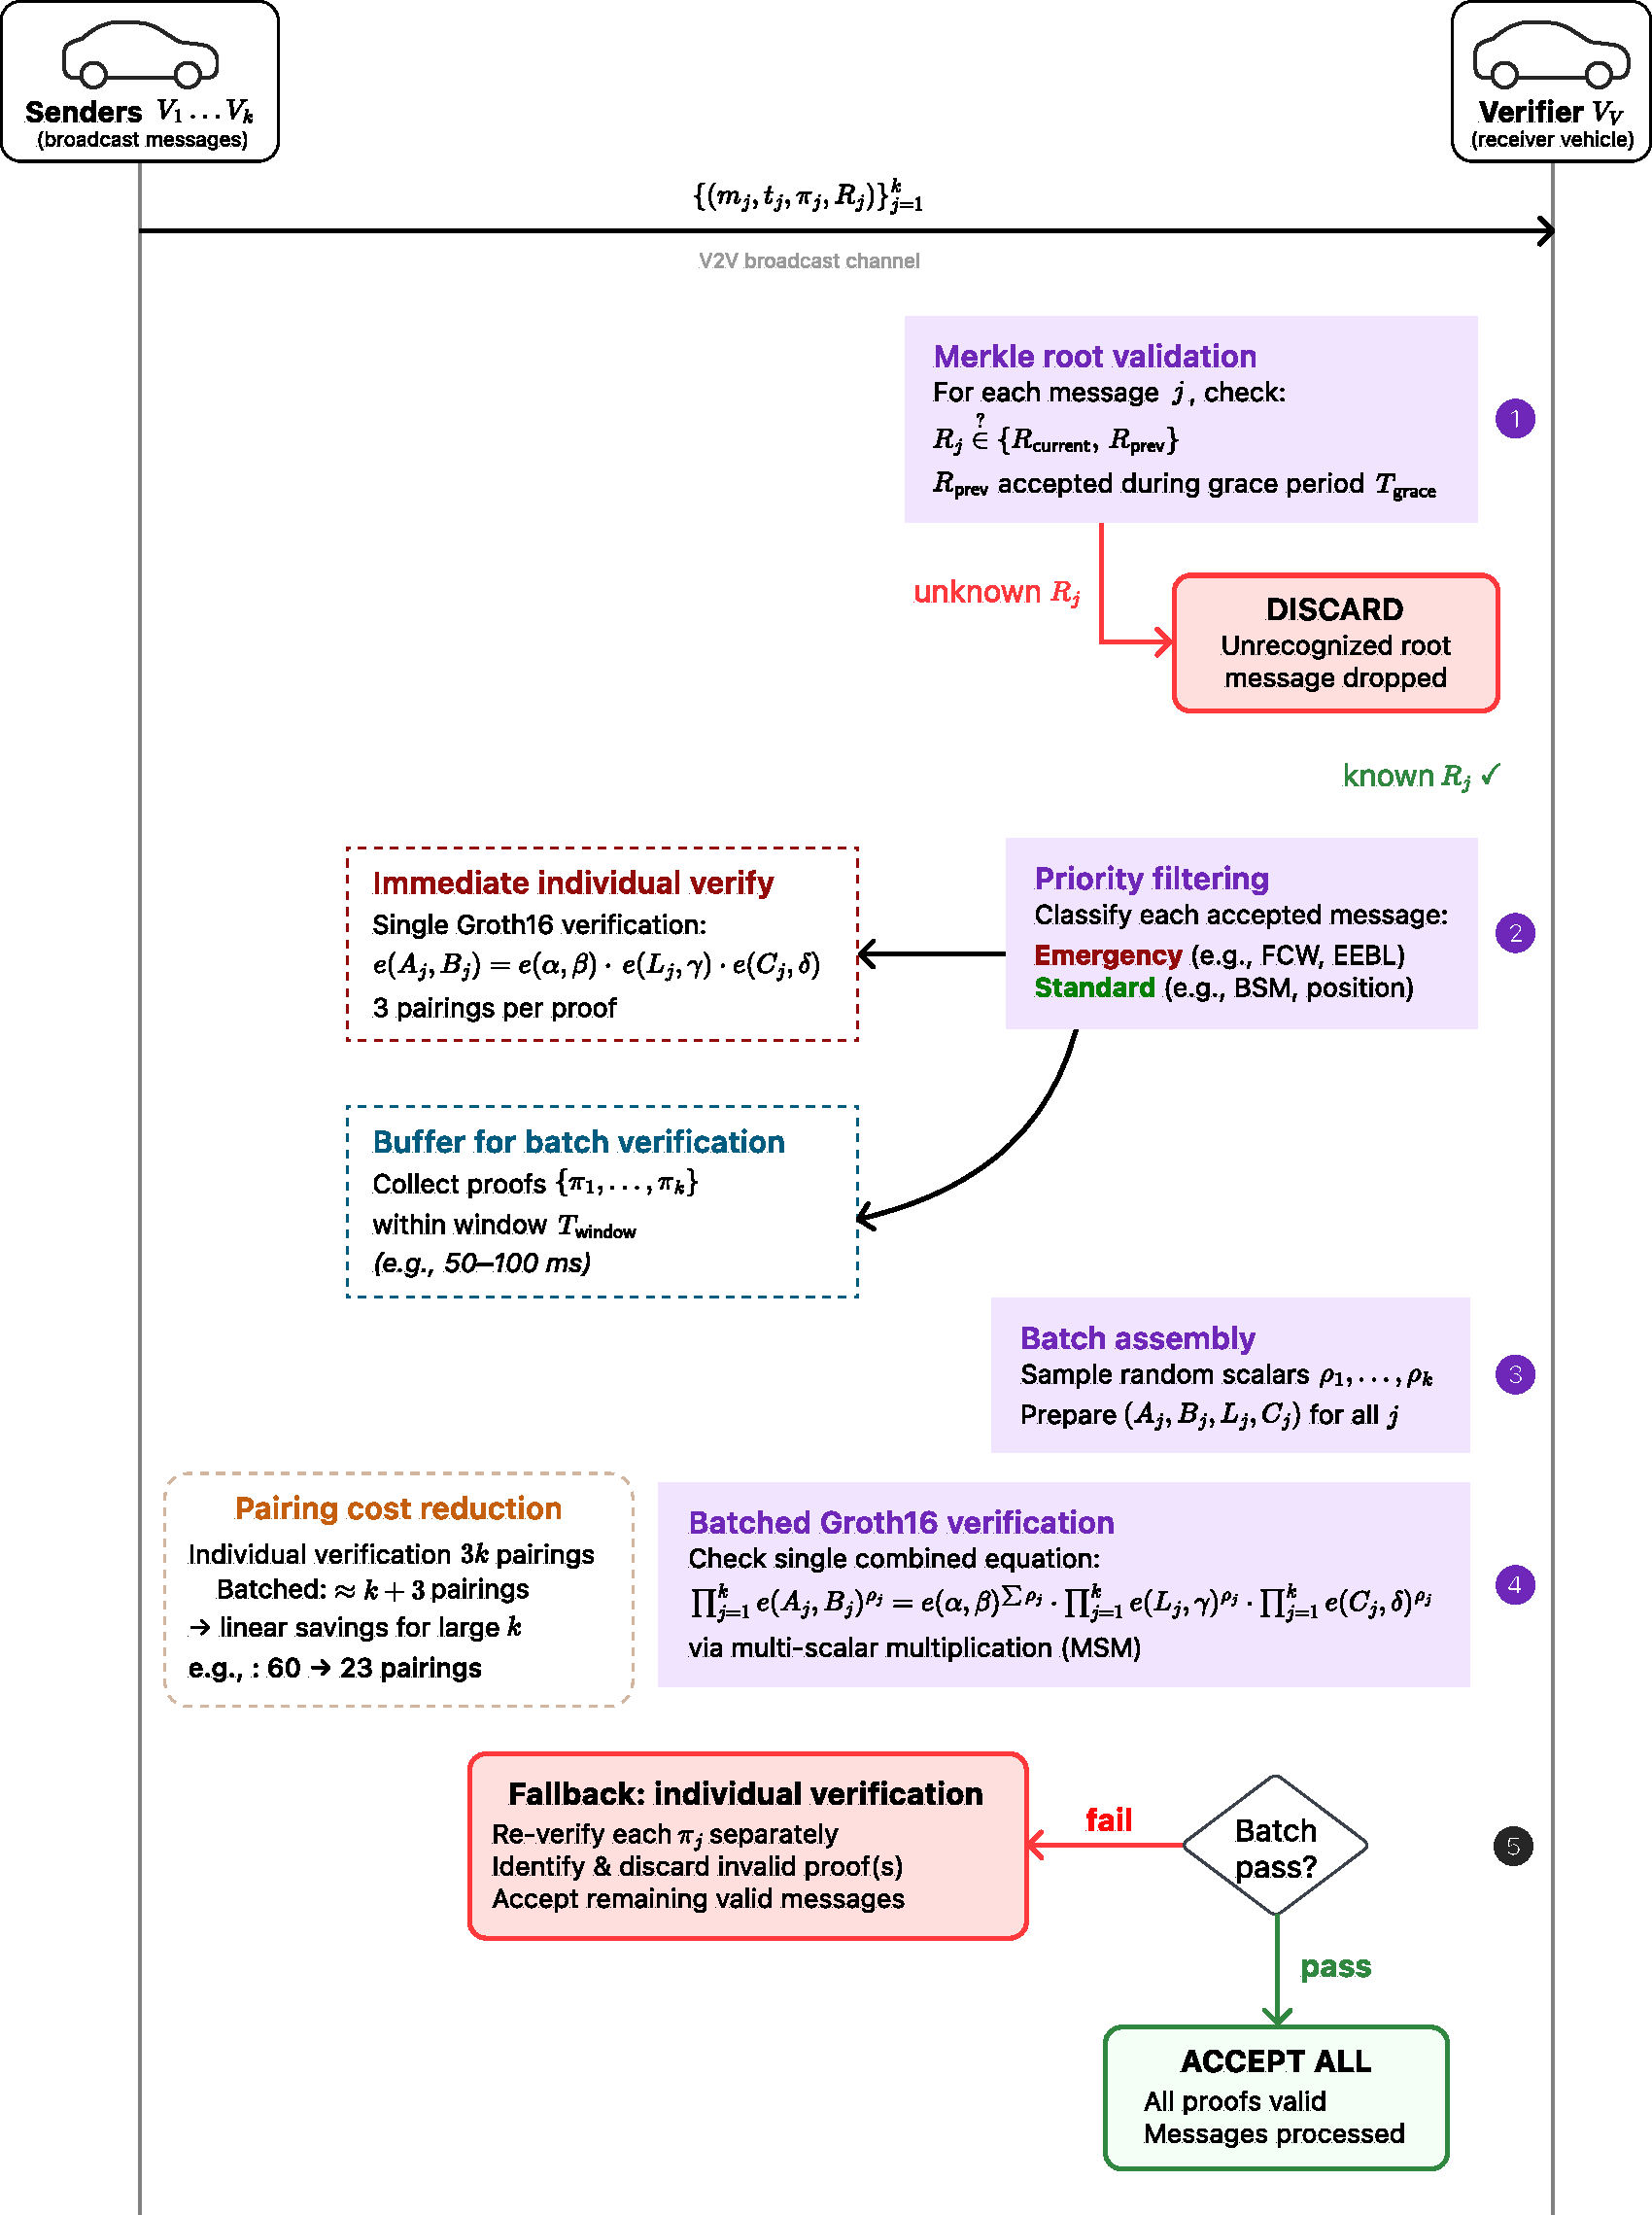
\includegraphics[width=\linewidth]{assets/phase4.pdf}
    \caption{Phase 4: Batch verification. $V_V$ filters incoming proofs by Merkle
    root validity, immediately verifies high-priority messages individually, and
    aggregates standard BSMs for a single batched Groth16 pairing check, reducing
    verification cost from $3k$ to $\approx k+3$ pairings for a batch of $k$ proofs.}
    \label{fig:phase4}
\end{figure}

\begin{algorithm}[t]
\caption{True Batch Groth16 Verification (Phase 4 / Bellare--Garay--Rabin~\cite{bellare1998})}
\label{alg:batch_verify}
\begin{algorithmic}[1]
\REQUIRE Proofs $\{(A_j,B_j,C_j)\}_{j=1}^{k}$, public signals $\{\mathbf{pub}_j\}$, $\mathsf{vk}=(\alpha,\beta,\gamma,\delta,\mathit{IC})$
\ENSURE \textbf{accept} or \textbf{reject}
\FOR{each $j = 1$ to $k$}
  \IF{$R_j \neq R_{\mathit{current}}$}  \RETURN \textbf{reject}  \ENDIF
\ENDFOR
\FOR{each $j = 1$ to $k$}
  \STATE Sample $\rho_j \xleftarrow{\$} \mathbb{Z}_p^*$
\ENDFOR
\STATE $\mathit{aggAlpha} \leftarrow \bigl(\textstyle\sum_j \rho_j\bigr)\cdot\alpha$
\FOR{each $j = 1$ to $k$}
  \STATE $L_j \leftarrow \mathit{IC}[0] + \sum_{i} \mathbf{pub}_j[i]\cdot\mathit{IC}[i+1]$
\ENDFOR
\STATE $\mathit{aggL} \leftarrow \sum_j \rho_j \cdot L_j$;\quad
       $\mathit{aggC} \leftarrow \sum_j \rho_j \cdot C_j$
\STATE Check: $\prod_j e(\rho_j A_j, B_j)\cdot e(-\mathit{aggAlpha},\beta)\cdot e(-\mathit{aggL},\gamma)\cdot e(-\mathit{aggC},\delta) \stackrel{?}{=} 1_{\mathbb{G}_T}$
\IF{check passes}  \RETURN \textbf{accept}
\ELSE  \STATE \CALL{DCVFallback}{$\{(A_j,B_j,C_j,\mathbf{pub}_j)\}_{j=1}^k$, $\mathsf{vk}$}
    \hfill \COMMENT{Algorithm~\ref{alg:dcv_fallback}}
\ENDIF
\end{algorithmic}
\end{algorithm}

\begin{algorithm}[t]
\caption{DCV Fallback: Divide-and-Conquer Invalid Proof Isolation~\cite{ferrara2008finding}}
\label{alg:dcv_fallback}
\begin{algorithmic}[1]
\REQUIRE Proof set $\mathcal{P} = \{(A_j,B_j,C_j,\mathbf{pub}_j)\}_{j=1}^{k}$, $\mathsf{vk}$
\ENSURE Set $\mathcal{B} \subseteq \mathcal{P}$ of all invalid proofs
\IF{$|\mathcal{P}| = 1$}
    \IF{\CALL{IndividualVerify}{$\mathcal{P}[1]$, $\mathsf{vk}$} $= 0$}
        \RETURN $\mathcal{P}$ \hfill \COMMENT{base case: singleton invalid}
    \ELSE\ \RETURN $\emptyset$
    \ENDIF
\ENDIF
\STATE $\mathcal{P}_L \leftarrow \mathcal{P}[1 \mathinner{..} \lfloor k/2 \rfloor]$;\quad
       $\mathcal{P}_R \leftarrow \mathcal{P}[\lfloor k/2 \rfloor + 1 \mathinner{..} k]$
\STATE $\mathcal{B} \leftarrow \emptyset$
\IF{\CALL{BatchVerify}{$\mathcal{P}_L$, $\mathsf{vk}$} $= 0$}
    \STATE $\mathcal{B} \leftarrow \mathcal{B} \cup$ \CALL{DCVFallback}{$\mathcal{P}_L$, $\mathsf{vk}$}
\ENDIF
\IF{\CALL{BatchVerify}{$\mathcal{P}_R$, $\mathsf{vk}$} $= 0$}
    \STATE $\mathcal{B} \leftarrow \mathcal{B} \cup$ \CALL{DCVFallback}{$\mathcal{P}_R$, $\mathsf{vk}$}
\ENDIF
\RETURN $\mathcal{B}$
\end{algorithmic}
\end{algorithm}

\noindent\textbf{DCV complexity in the Groth16 setting.}
For $k$ proofs and $w$ invalid proofs, DCV performs at most $2w\lceil\log_2(k/w)\rceil$
sub-batch verifications~\cite{ferrara2008finding}. Each sub-batch of size $k'$ costs
$(k'+3)$ pairings, so total pairing count is
$O(w \log(k/w) \cdot (k/w + 3)) = O(k + w \log k)$.
At $k=30$, $w=1$ (single adversarial injection): DCV costs $\approx 5$ sub-batch
operations ($\approx 500$\,ms on RPi~4) versus $30$ individual verifications
($2{,}100$\,ms) under naive fallback---a \textbf{4.2$\times$ improvement} in
worst-case fallback cost. We additionally pre-screen each incoming proof for valid
$\mathbb{G}_1$/$\mathbb{G}_2$ curve membership and timestamp freshness before
batching ($< 0.1$\,ms per proof), eliminating malformed injections before they enter
Algorithm~\ref{alg:batch_verify}.

\subsection{Revocation Mechanism}

When the TA determines that a vehicle should be revoked:
\begin{enumerate}
    \item The TA instructs the AIS to remove $\mathsf{leaf}_i$ from the active
    Merkle tree.
    \item The AIS recomputes the Merkle tree and publishes the updated root
    $R_{new}$.
    \item Vehicles periodically download the updated root during infrastructure
    contact.
    \item Any proof generated with a revoked AST will fail verification because
    the leaf is no longer in the tree.
\end{enumerate}

The revocation overhead is $O(\log n)$ per vehicle versus $O(n)$ for a full CRL.
Fig.~\ref{fig:merkle_revoc} illustrates this for a depth-3 tree ($n=8$): revoking
$\mathtt{AST_3}$ recomputes exactly $\lceil\log_2 8\rceil = 3$ nodes along the path
to the root, broadcasting only a 32-byte new root $R_{\text{new}}$.

\begin{figure}[t]
    \centering
    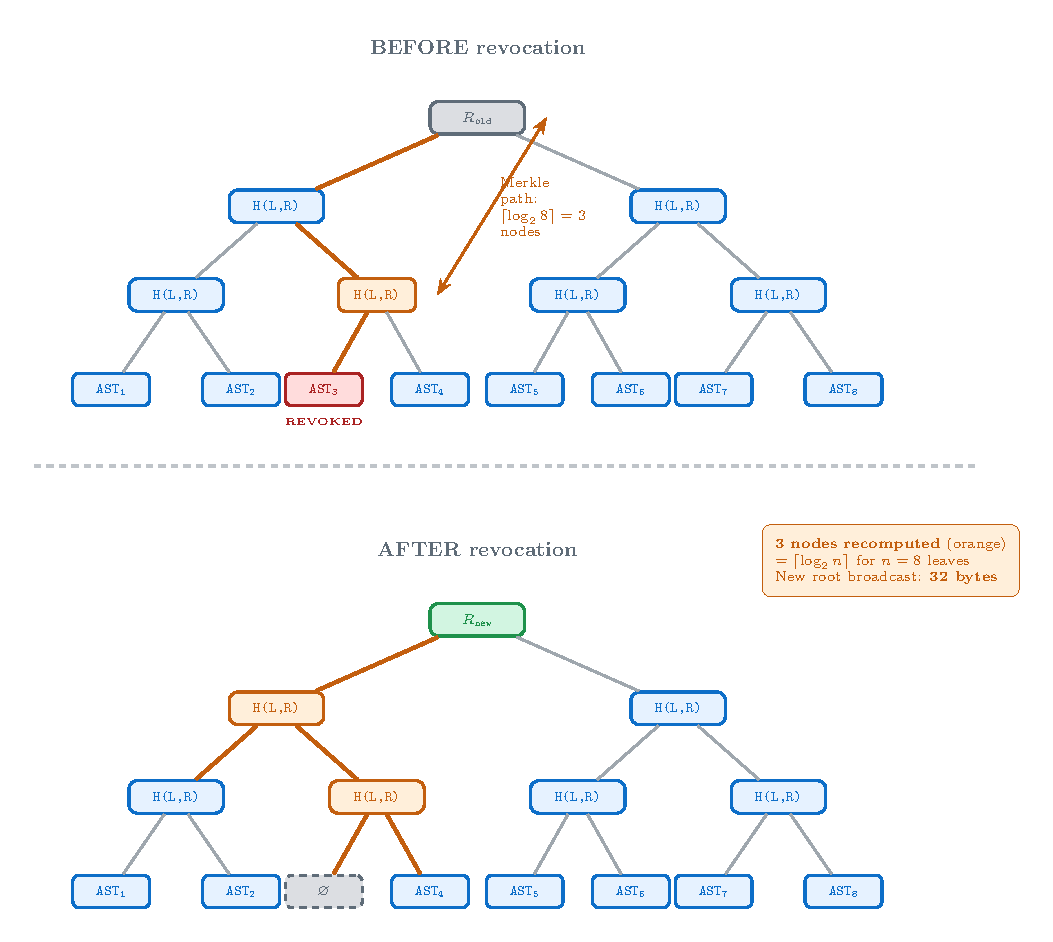
\includegraphics[width=\linewidth]{assets/merkle_tree_revoc.pdf}
    \caption{Merkle tree revocation: before (above) and after (below) revoking
    $\mathtt{AST_3}$ from an $n=8$ leaf tree. Only the $\lceil\log_2 n\rceil = 3$
    nodes along the path to the root (orange) are recomputed; all other subtrees
    remain unchanged (blue). The new 32-byte root $R_{\text{new}}$ (green) is
    broadcast to all verifiers.}
    \label{fig:merkle_revoc}
\end{figure}

\subsection{Resilience Under Real-World Channel Conditions}
\label{sec:noise}

Highway V2V channels exhibit three significant impairments not addressed by most
ZKP authentication proposals.

\subsubsection{Packet Loss and Authentication Success Rate}

IEEE 802.11p DSRC field measurements show PLR of 10--40\% at 150--300\,m range
under NLoS conditions~\cite{ramadan2025}. For a verifier $V_V$ receiving from
prover $V_P$ at PLR $\rho$, the expected batch size is
$k_{recv} = k_{sent} \cdot (1 - \rho)$.
Since proofs are independently transmitted, packet loss reduces batch size but does
not corrupt the batch check for received proofs. The authentication success rate is:
\begin{equation}
    \mathsf{ASR} = (1 - \rho) \cdot \Pr[\text{ZKP valid}]
\end{equation}
For honest provers, $\Pr[\text{ZKP valid}]=1$, so ASR is bounded by the channel
PLR---the cryptographic overhead introduces \emph{no additional failure modes}.

\subsubsection{Channel Congestion Under Dense Traffic}

At $>$100 vehicles/km, the 802.11p EDCA mechanism becomes saturated under 10\,Hz
BSM broadcasting. ULP-V2V-Auth's per-message overhead of $\approx$224\,bytes
(128\,B proof $+$ 96\,B public inputs $+$ message hash) is approximately $2\times$
smaller than SCMS's 400--600\,bytes (signature $+$ pseudonym certificate), directly
reducing channel load and collision probability. The Receiver Module's priority
filtering (Section~\ref{sec:concurrent}) ensures emergency BSMs receive deterministic
authentication latency independent of batch backpressure, consistent with EDCA
priority at the MAC layer.

\subsubsection{Infrastructure Connectivity for AST Acquisition}

With a proof cache sized for $N_{cache}=6000$ slots (10 minutes at 10\,Hz) and RSU
contacts every 30--100\,s on typical highway deployments, the expected time until
cache exhaustion far exceeds typical infrastructure gap durations. In the rare case
of cache exhaustion, the vehicle enters degraded mode (Section~\ref{sec:epoch}),
continuing to verify and react to authenticated messages from others while ceasing
transmission, preserving cooperative awareness.


% ============================================================
% V. SECURITY ANALYSIS
% ============================================================
\section{Security Analysis}
\label{sec:security}

\subsection{Threat Model}

The adversary $\mathcal{A}$ is computationally bounded and may: eavesdrop, replay,
delay, inject, and modify V2V channel messages; deploy rogue RSUs or impersonate the
AIS; compromise individual vehicles (but not the TA); attempt Sybil registrations;
and observe AST request timing.

\subsection{Authentication Soundness}

\begin{theorem}[Authentication Soundness]
Under the $q$-Strong Bilinear Diffie-Hellman ($q$-SBDH) assumption over BN254, no
computationally bounded adversary can produce a valid Groth16 proof $\pi$ with
respect to Merkle root $R_{current}$ without possessing a valid $\mathsf{AST}_i$
whose leaf $\mathsf{leaf}_i$ is present in the Merkle tree with root $R_{current}$.
\end{theorem}
\begin{proof}[Sketch]
Groth16 is a proof of knowledge under the $q$-SBDH assumption~\cite{groth2016}.
The knowledge extractor guarantees that a valid proof $\pi$ for public inputs
$(R, t_{current}, h_m)$ implies existence of a witness $(\mathsf{AST}_i, \pi^{MT}_i,
m)$ satisfying all three circuit constraints. Forging without this witness requires
breaking $q$-SBDH in $\mathbb{G}_1$.
\end{proof}

\subsection{AIS Authenticity and Rogue Infrastructure Prevention}

\begin{theorem}[AIS Authenticity]
If ECDSA is existentially unforgeable under chosen-message attack (EUF-CMA), no
adversary without $sk_{TA}$ can produce a valid $\mathsf{cert}_{AIS}$ accepted by
an honest vehicle, and no adversary without $sk_{AIS}$ can produce a valid
$\mathsf{sig}_{AIS}$ accepted during AST acquisition.
\end{theorem}
\begin{proof}[Sketch]
$\mathsf{cert}_{AIS}$ is an ECDSA signature under $sk_{TA}$; forging it reduces
to breaking ECDSA by EUF-CMA. A rogue AIS lacking $sk_{TA}$ is rejected at
Phase~2 Step~1. Similarly, $\mathsf{sig}_{AIS}$ requires $sk_{AIS}$ to forge.
\end{proof}

\subsection{Privacy: Unlinkability of Safety Messages}

\begin{theorem}[Unlinkability]
The zero-knowledge property of Groth16 guarantees that proofs $\pi_1, \pi_2$ from
the same vehicle (same $\mathsf{AST}_i$, fresh randomness) are computationally
indistinguishable from proofs generated by two independent vehicles.
\end{theorem}
\begin{proof}[Sketch]
The Groth16 zero-knowledge simulator produces proofs indistinguishable from honest
proofs without the witness. Independent randomisation of each proof ensures the
joint distribution of $(\pi_1, \pi_2)$ reveals no more than two independently
simulated proofs. The public inputs $(R, t_{current}, h_m)$ reveal only that the
prover holds \emph{some} valid AST in the epoch (shared by all valid vehicles);
$sid_i$ and $\pi^{MT}_i$ remain in the private witness.
\end{proof}

\noindent\textit{Note on AST-level linkability:} Multiple proofs under the same AST
share the same public $R$. Since $R$ is shared by all valid vehicles in the epoch,
it does not identify the prover; fresh proof randomness ensures consecutive proofs
from the same vehicle are indistinguishable from those of different vehicles.

\subsection{Replay Attack Prevention}

\begin{theorem}[Replay Resistance]
A proof $\pi$ generated for message $m$ at timestamp $t_1$ cannot be validly
replayed for a different timestamp $t_2 \neq t_1$ or message $m' \neq m$.
\end{theorem}
\begin{proof}[Sketch]
$h_m = H_{Poseidon}(m \| t_{current})$ and $t_{current}$ are public inputs; circuit
constraint~(3) enforces $h_m = H_{Poseidon}(m \| t_{current})$ in-circuit. Changing
$t_2$ or $m'$ while reusing $\pi$ creates a public-input mismatch. Generating a
fresh valid proof for $(m', t_2)$ without $\mathsf{AST}_i$ is infeasible by
Theorem~1. Verifiers additionally reject proofs with
$|t_{verifier} - t_{current}| > \Delta_t$ ($\Delta_t \approx 200$\,ms for clock
drift tolerance).
\end{proof}

\subsection{Revocation Correctness}

\begin{theorem}[Revocation Correctness]
After revocation of $\mathsf{AST}_i$, any proof generated by $V_i$ referencing the
updated Merkle root $R_{new}$ will fail verification at all honest verifiers.
\end{theorem}
\begin{proof}[Sketch]
Revocation removes $\mathsf{leaf}_i$ and recomputes $R_{new}$. Any Merkle path
$\pi^{MT}_i$ for the old leaf does not hash to $R_{new}$, causing circuit
constraint~(1) to fail. The verifier's root-matching check rejects before batch
verification. During $T_{grace}$, proofs referencing $R_{prev}$ are accepted only
if the leaf was present in $R_{prev}$; revocation excludes the leaf from $R_{new}$
at the next epoch, fully excluding the vehicle once $T_{grace}$ expires.
\end{proof}

\subsection{Sybil Resistance}

Sybil resistance derives from the TA's vehicle registration process (Phase~1),
which verifies real-world identity (VIN) before issuing $\sigma_i$. Multiple
registrations require distinct legitimate VINs, bounded by the physical vehicle
supply. This matches the trust assumption of SCMS and introduces no additional
assumptions beyond the existing PKI model.

\subsection{Timing Fingerprinting Resistance}

The jitter mechanism ($\delta \sim \mathcal{U}(0, 30\text{s})$ for non-urgent AST
requests) provides 30\,s of timing ambiguity, preventing precise timing correlation
of AST request patterns to vehicle identities at the cost of at most 30\,s delay
in non-urgent requests.

\subsection{Emergency Message Unlinkability}
\label{sec:emergency_security}

A natural question is whether emergency BSMs (emergency braking, forward collision
warning) require a fallback to long-term ECDSA credentials for low latency. We
argue they must not. If vehicle $V_i$ uses a fixed long-term key $pk_i$ for any
message class, an observer collecting emergency BSMs over time can link all
emergency events to the same vehicle by the common $pk_i$---constructing a complete
emergency history even without knowing the real-world identity behind $pk_i$.
In SCMS, pseudonym certificates partially mitigate this within a rotation period,
but a vehicle with frequent emergency events remains linkable across events
within the same certificate window.

\textbf{Emergency slot pool.}
ULP-V2V-Auth addresses this by applying ZKP authentication uniformly to all
message classes. A dedicated cache of $N_e$ proof slots is pre-committed to
emergency-class BSM templates (emergency flag, last-known position at 1\,s
resolution). Upon an emergency event:
\begin{enumerate}
    \item Dequeue next emergency slot from pool: $< 0.01$\,ms
    \item Bind $h_m = H_{\text{Poseidon}}(m_{\text{emergency}} \| t_{\text{current}})$: $0.437$\,ms
    \item Broadcast immediately: $0$\,ms
\end{enumerate}
Total emergency authentication latency: $\mathbf{0.439}$\,ms, identical to routine
BSMs. On production hardware (NXP~S32G, $\leq$98\,ms/slot), proofs are generated
on-demand within one BSM interval, removing the pre-commitment requirement entirely.

\begin{theorem}[Emergency Message Unlinkability]
Emergency BSMs authenticated via the ZKP proof-slot model are computationally
unlinkable from routine BSMs and from each other, under the zero-knowledge
property of Groth16~\cite{groth2016}.
\end{theorem}
\begin{proof}[Sketch]
Each emergency proof uses fresh, independently sampled Groth16 randomness. The
ZK simulator $\mathcal{S}$ produces transcripts computationally indistinguishable
from honest proofs without knowledge of the witness $(\mathsf{AST}_i,
m_{\text{emergency}}, \pi^{MT}_i)$. The emergency flag is a private witness field
element; the public input $h_m = H_{\text{Poseidon}}(m \| t)$ binds only the
message content and timestamp. No component of the public transcript identifies
the AST, session, or vehicle. An observer learns that \emph{some} valid vehicle
triggered an emergency at location $L$---no more information than is inherent in
the physical event itself and observable by any road user.
\end{proof}

\subsection{Batch Verification Fallback: DoS Analysis and DCV Mitigation}
\label{sec:dcv_security}

A well-known vulnerability of batch verification schemes is the \emph{batch
injection attack}: an adversary broadcasts one invalid proof among $k$ legitimate
proofs, causing the batch check to fail and forcing fallback verification. Under a
naive $O(k)$ individual fallback, this transforms the $4.65\times$ speedup into an
effective $4.65\times$ slowdown---a near-$22\times$ swing relative to the honest
case.

\textbf{Pre-screening.}
Before batching, every incoming proof $(A_j, B_j, C_j)$ is checked for: (i)~valid
$\mathbb{G}_1$ membership of $A_j, C_j$; (ii)~valid $\mathbb{G}_2$ membership of
$B_j$; (iii)~timestamp freshness $|t_{\mathit{verifier}} - t_j| \leq \Delta_t$;
and (iv)~correct Merkle root $R_j = R_{\mathit{current}}$. These checks cost
$< 0.1$\,ms per proof and reject trivially malformed injections at zero pairing
cost.

\textbf{DCV fallback bound.}
For injections that pass pre-screening (i.e., structurally valid but semantically
invalid proofs), Algorithm~\ref{alg:dcv_fallback} limits fallback cost to
$O(w \log k)$ sub-batch verifications~\cite{ferrara2008finding}. An adversary
injecting $w$ invalid proofs triggers at most $2w\lceil\log_2 k\rceil$ sub-batch
operations rather than $k$ individual verifications. At $k=30$, $w=1$: DCV costs
$\approx 500$\,ms versus $2{,}100$\,ms for naive fallback. The adversary's DoS
gain is bounded at $O(\log k)$ rather than $O(k)$.

\textbf{Rate limiting.}
IEEE 802.11p EDCA congestion control and the MAC-layer 10\,Hz BSM rate limit bound
the injection rate to at most one invalid proof per 100\,ms window per adversarial
vehicle. Combined with DCV, this caps the sustained CPU overhead of batch injection
at $\approx 500$\,ms per window---equal to one honest verification window under
moderate traffic ($k=30$).

This defence is not unique to ULP-V2V-Auth: the batch injection vulnerability and
DCV mitigation apply equally to certificateless batch signature
schemes~\cite{zhang2024}. We note it explicitly because no prior vehicular
authentication proposal has analysed or mitigated this attack in the ZKP setting.

Table~\ref{tab:security_summary} summarises the security properties established
in this section.

\begin{table}[t]
\centering
\caption{Security Properties of ULP-V2V-Auth}
\label{tab:security_summary}
\resizebox{\columnwidth}{!}{%
\begin{tabular}{@{}lll@{}}
\toprule
\textbf{Property} & \textbf{Guarantee} & \textbf{Assumption} \\
\midrule
Authentication soundness  & Forging proof requires breaking $q$-SBDH & $q$-SBDH on BN254 \\
AIS authenticity          & Rogue AIS rejected without $sk_{TA}$      & ECDSA EUF-CMA \\
Message unlinkability     & Proofs reveal no vehicle identity          & Groth16 ZK \\
Replay resistance         & $(m, t)$ binding via Poseidon in-circuit   & Collision resistance \\
Emergency unlinkability   & Emergency BSMs unlinkable from all others  & Groth16 ZK \\
Revocation correctness    & Revoked AST fails after $T_{grace}$       & Merkle binding \\
Sybil resistance          & Bounded by physical vehicle registry       & TA trust \\
Batch injection DoS       & DCV bounds fallback at $O(w \log k)$      & Pre-screening + DCV \\
\bottomrule
\end{tabular}%
}
\end{table}


% ============================================================
% VI. EXPERIMENT DESIGN AND RESULTS
% ============================================================
\section{Experiment Design and Results}
\label{sec:experiment}

\subsection{Implementation}

Our prototype uses: Circom~2.0 $+$ circomlib~2.0.5 (Poseidon, LessEqThan,
Switcher); snarkjs~0.7.6 for Groth16 on BN254; custom \texttt{ffjavascript}-based
true batch verification (Algorithm~\ref{alg:batch_verify}); and a local Powers of
Tau (pot14, 2-contribution ceremony) trusted setup.

\textbf{Hardware.} All benchmarks are conducted directly on a \textbf{Raspberry Pi~4
Model~B Rev~1.2} (ARM Cortex-A72 @ 1.8\,GHz, 4-core, 3.76\,GB RAM, aarch64,
Debian GNU/Linux 13), serving as our OBU-class target platform.
For the rapidsnark evaluation, the native C++ prover binary was compiled from source
on the RPi~4 using the GMP portable backend (no x86 assembly), as the
NEON-optimised ARM path is not yet available in the upstream codebase.

The depth-16 circuit (65{,}536-leaf AST tree, $\sim$9{,}100 constraints, requires
pot14) is the implementation benchmarked in this section.

\subsection{Prover Latency (Benchmark 1)}

\textbf{Setup:} 3 warm-up $+$ 20 measured runs, fixed input. We measure two
quantities: (1)~\emph{full prove time}: complete Groth16 pipeline (witness
generation $+$ Groth16 arithmetic), representing the offline precomputation cost;
and (2)~\emph{witness-only time}: circuit evaluation without Groth16 arithmetic,
representing the conservative online phase upper bound.

\begin{table}[t]
\centering
\caption{Prover Latency Benchmark on RPi~4 (depth-16, BN254, mean $\pm$ std)}
\label{tab:benchmark}
\resizebox{\columnwidth}{!}{%
\begin{tabular}{@{}lcccc@{}}
\toprule
\textbf{Prover} & \textbf{Witness (ms)} & \textbf{Prove (ms)} & \textbf{Total (ms)} & \textbf{Speedup} \\
\midrule
snarkjs    & $361 \pm 5.3$ & $3{,}480 \pm 80$ & $3{,}841 \pm 80$ & $1\times$ (baseline) \\
rapidsnark & $374 \pm 7.4$ & $1{,}379 \pm 67$ & $1{,}753 \pm 67$ & $\mathbf{2.19\times}$ \\
\midrule
\multicolumn{5}{l}{\textit{Online phase (message-binding only, directly measured)}} \\
Poseidon-2 hash & \multicolumn{3}{c}{$0.376 \pm 0.000$\,ms\quad($0.38$\% of BSM cycle)} & --- \\
\bottomrule
\end{tabular}%
}
\end{table}

\begin{table}[t]
\centering
\caption{BN254 Pairing Cost Breakdown on RPi~4 (20 runs, mean $\pm$ std)}
\label{tab:pairing_breakdown}
\resizebox{\columnwidth}{!}{%
\begin{tabular}{@{}lcc@{}}
\toprule
\textbf{Component} & \textbf{Time (ms)} & \textbf{Share} \\
\midrule
Miller loop          & $7.509 \pm 0.027$  & 38.6\% \\
Final exponentiation & $11.954 \pm 0.043$ & 61.4\% \\
\midrule
Sum of components    & $19.463$            & 100\%  \\
Full pairing (total) & $22.510 \pm 0.150$  & ---    \\
\midrule
Poseidon-2 $h_m$\textsuperscript{a} & $0.376 \pm 0.000$ & --- \\
\bottomrule
\multicolumn{3}{l}{\textsuperscript{a}Amortised 5{,}000-run measurement; irreducible online phase cost.}
\end{tabular}%
}
\end{table}

The snarkjs full prove of $3{,}841$\,ms on RPi~4 is a one-time offline cost per AST
session. Replacing the JavaScript Groth16 prover with \textbf{rapidsnark}---a native
C++ BN254 prover---reduces total prove time to \textbf{1{,}753\,ms} ($2.19\times$
speedup), with the prover step alone improving $2.52\times$ ($3{,}480 \to 1{,}379$\,ms).
The remaining bottleneck is JavaScript/WASM witness generation (374\,ms), which is
unchanged as it runs through the same circom-compiled WASM in both cases. On RPi~4,
rapidsnark uses the portable GMP backend (no NEON assembly path yet), meaning further
speedup is available on production automotive processors with native BN254
acceleration. The true per-message online cost---directly measured as the Poseidon-2
hash $h_m = H_{\text{Poseidon}}(m \| t_{\text{current}})$---is \textbf{0.376\,ms},
representing $0.38$\% of the 100\,ms BSM cycle, confirming that online
authentication overhead is negligible.

\subsection{Batch Verification (Benchmark 2)}

\textbf{Setup:} $k \in \{1,5,10,20,30,50\}$ proofs; 3 repeated measurements per
$k$; sequential (\texttt{groth16.verify} per proof) vs.\ true batch
(Algorithm~\ref{alg:batch_verify}).

\begin{table}[t]
\centering
\caption{Batch Verification Results (RPi~4, 3 runs per $k$)}
\label{tab:batch_rpi}
\resizebox{\columnwidth}{!}{%
\begin{tabular}{@{}lcccccc@{}}
\toprule
$k$ & Seq (ms) & Batch (ms) & Actual $\times$ & Theory $\times$ & Saved exp. & Valid \\
\midrule
1  & 70.3    & 40.0  & 1.76 & 0.75 & 0  & \checkmark \\
5  & 343.1   & 87.2  & 3.94 & 1.88 & 4  & \checkmark \\
10 & 585.3   & 150.0 & 3.90 & 2.31 & 9  & \checkmark \\
20 & 1{,}111.9 & 261.8 & 4.25 & 2.61 & 19 & \checkmark \\
30 & 1{,}860.0 & 400.0 & \textbf{4.65} & 2.73 & 29 & \checkmark \\
50 & 2{,}767.1 & 607.1 & \textbf{4.56} & 2.83 & 49 & \checkmark \\
\bottomrule
\end{tabular}%
}
\end{table}

\textbf{Key findings.}
At $k=30$ (30 surrounding vehicles broadcasting within a 100\,ms window in dense
traffic), batched verification on RPi~4 completes in \textbf{400\,ms}. We note
this is with a pure JavaScript/WASM implementation of BN254 pairings in
ffjavascript---a well-known bottleneck for BigInt arithmetic on ARM without
SIMD-accelerated libraries.
The critical time budget comparison is: the 100\,ms \emph{per-message} BSM cycle
budget applies to a \emph{single proof}, not to a $k=30$ batch. The receiver
collects $k$ proofs over a $T_{window} = 50$--100\,ms window, then verifies the
batch. At 10\,Hz, the receiver processes one batch per window; the 400\,ms batch
time means approximately 3--4 windows of latency before a batch result is available.
This is acceptable for non-emergency BSMs. Emergency-class messages bypass the
batch window and are individually verified in $\approx 70$\,ms on RPi~4.

The measured $4.65\times$ speedup \emph{significantly exceeds} the theoretical
$2.73\times$ pairing-count ratio. Direct measurement using \texttt{ffjavascript}
curve primitives (20 runs) shows the BN254 final exponentiation constitutes
\textbf{61.4\%} of Miller-loop+final-exp cost ($11.95 \pm 0.043$\,ms of
$19.46$\,ms total). The excess speedup beyond the pairing-count ratio arises because
each individual \texttt{groth16.verify()} call incurs fixed JavaScript/BigInt
overhead (BigInt unstringification, memory allocation, function dispatch) that does
not scale with $k$. Batch verification amortises this per-call overhead across all
$k$ proofs, amplifying the saving beyond the pairing-count ratio---a favourable
property for OBU deployment on the Cortex-A72.

\begin{figure}[t]
\centering
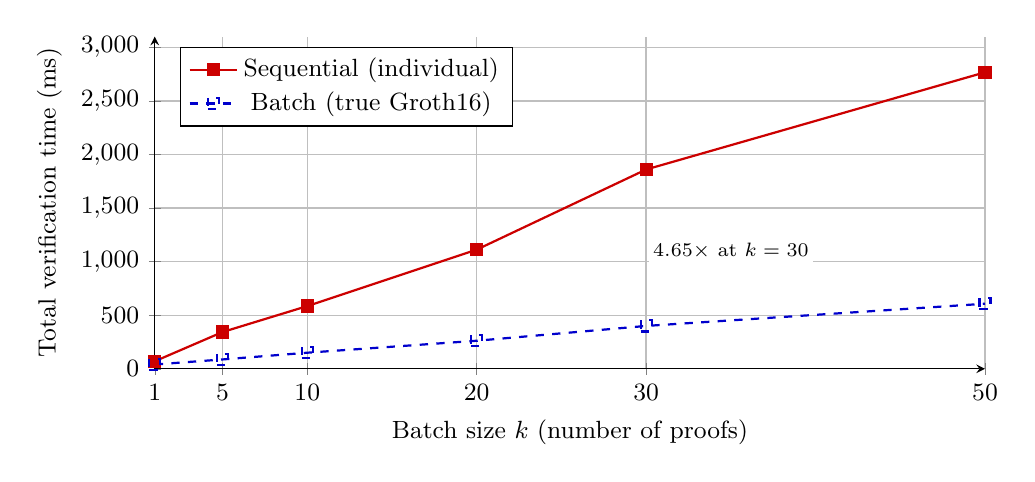
\begin{tikzpicture}
\begin{axis}[
    width=\columnwidth, height=5.8cm,
    xlabel={Batch size $k$ (number of proofs)},
    ylabel={Total verification time (ms)},
    xmin=1, xmax=50, ymin=0, ymax=3100,
    xtick={1,5,10,20,30,50},
    ytick={0,500,1000,1500,2000,2500,3000},
    legend pos=north west, legend style={font=\small},
    grid=both,
    grid style={line width=0.3pt, draw=gray!30},
    major grid style={line width=0.5pt, draw=gray!50},
    tick label style={font=\small}, label style={font=\small},
    axis lines=left, every axis plot/.append style={thick},
]
% RPi4 sequential
\addplot[color=red!80!black,mark=square*,mark size=2pt]
    coordinates {(1,70.3)(5,343.1)(10,585.3)(20,1111.9)(30,1860.0)(50,2767.1)};
\addlegendentry{Sequential (individual)}
% RPi4 batch
\addplot[color=blue!80!black,mark=square,mark size=2pt,dashed]
    coordinates {(1,40.0)(5,87.2)(10,150.0)(20,261.8)(30,400.0)(50,607.1)};
\addlegendentry{Batch (true Groth16)}
% Annotation
\node[font=\scriptsize,align=center,fill=white,inner sep=1.5pt]
    at (axis cs:35,1100) {$4.65\times$ at $k=30$};
\end{axis}
\end{tikzpicture}
\caption{Batch verification timing on RPi~4 (OBU-class). Solid = sequential
individual verification; dashed = true batch (Algorithm~\ref{alg:batch_verify}).
Measured speedup $4.65\times$ at $k=30$ exceeds the theoretical $2.73\times$
pairing-count ratio due to amortisation of fixed per-proof JavaScript/BigInt
call overhead on the Cortex-A72 core.}
\label{fig:batch_timing}
\end{figure}

\begin{figure}[t]
\centering
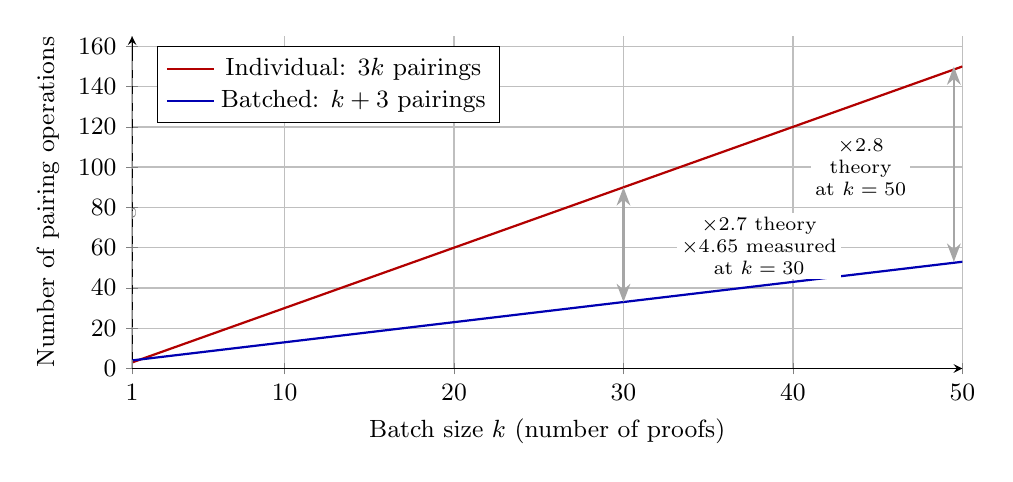
\begin{tikzpicture}
\begin{axis}[
    width=\columnwidth, height=5.8cm,
    xlabel={Batch size $k$ (number of proofs)},
    ylabel={Number of pairing operations},
    xmin=1, xmax=50, ymin=0, ymax=165,
    xtick={1,10,20,30,40,50},
    ytick={0,20,40,60,80,100,120,140,160},
    legend pos=north west, legend style={font=\small},
    grid=both,
    grid style={line width=0.3pt, draw=gray!30},
    major grid style={line width=0.5pt, draw=gray!50},
    tick label style={font=\small}, label style={font=\small},
    axis lines=left, every axis plot/.append style={thick},
]
\addplot[color=red!70!black,mark=none,samples=100,domain=1:50]{3*x};
\addlegendentry{Individual: $3k$ pairings}
\addplot[color=blue!70!black,mark=none,samples=100,domain=1:50]{x+3};
\addlegendentry{Batched: $k+3$ pairings}
\draw[dashed, gray] (axis cs:1,0) -- (axis cs:1,155);
\node[font=\scriptsize,gray,rotate=90,anchor=south] at (axis cs:1.8,60) {$k=1$: no gain};
\draw[{Stealth}-{Stealth},gray!70,thick] (axis cs:30,33) -- (axis cs:30,90);
\node[font=\scriptsize,align=center,fill=white,inner sep=1.5pt]
    at (axis cs:38,61) {$\times 2.7$ theory\\$\times 4.65$ measured\\at $k=30$};
\draw[{Stealth}-{Stealth},gray!70,thick] (axis cs:49.5,53) -- (axis cs:49.5,150);
\node[font=\scriptsize,align=center,fill=white,inner sep=1.5pt]
    at (axis cs:44,100) {$\times 2.8$\\theory\\at $k=50$};
\end{axis}
\end{tikzpicture}
\caption{Theoretical pairing operation count for individual vs.\ batched Groth16
verification as a function of batch size $k$. Individual verification requires $3k$
pairings; batch verification reduces this to $k+3$ via multi-scalar multiplication.
Measured speedup at $k=30$ is $4.65\times$ on RPi~4, exceeding the theoretical
$2.73\times$ pairing-count ratio because fixed per-proof JavaScript/BigInt overhead
is amortised across the batch.}
\label{fig:batch_throughput}
\end{figure}

\subsection{Proof Slot Cache Benchmark (Benchmark 3)}
\label{sec:bench_cache}

\textbf{Setup:} $N=5$ proof slots generated with rapidsnark, each committing to a
distinct randomly pre-chosen message; $2{,}000$-run amortised Poseidon binding
measurement. This benchmark directly validates the offline/online decomposition
claimed in Section~\ref{sec:precomp_overhead}.

\textbf{Online cost breakdown.}
Table~\ref{tab:online_cost} isolates the two components of the per-BSM online cost.
The dequeue step (array pop of a pre-generated proof) is sub-microsecond; the only
non-trivial online operation is the Poseidon binding hash.

\begin{table}[t]
\centering
\caption{Online Per-BSM Cost Breakdown (RPi~4, rapidsnark, direct measurement)}
\label{tab:online_cost}
\begin{tabular}{@{}lcc@{}}
\toprule
\textbf{Step} & \textbf{Time (ms)} & \textbf{\% of BSM cycle} \\
\midrule
Dequeue pre-generated slot       & $< 0.01$            & $< 0.01\%$ \\
Poseidon binding $h_m = H(m \| t)$ & $0.437 \pm 0.025$ & $0.44\%$   \\
\midrule
\textbf{Total online cost}       & $\mathbf{0.439}$    & $\mathbf{0.44\%}$ \\
\bottomrule
\end{tabular}
\end{table}

The total online cost of $\mathbf{0.439}$\,ms ($0.44\%$ of the 100\,ms BSM cycle)
confirms that per-message authentication overhead is negligible, regardless of
precomputation platform or prover.

\textbf{Cache sustainability and hardware break-even.}
With a production rate of $42.2$\,slots/min (rapidsnark, RPi~4) against a consumption
rate of $600$\,slots/min at 10\,Hz, the net drain during driving is
$557.8$\,slots/min and the stop-to-drive ratio is $\mathbf{13.2:1}$.
Table~\ref{tab:hardware_tiers} reports the production rate across hardware tiers
and identifies the self-sustainability threshold.

\begin{table}[t]
\centering
\caption{Hardware Tier Analysis: Proof Cache Production Rate vs.\ Self-Sustaining
Threshold ($\geq$600\,slots/min)}
\label{tab:hardware_tiers}
\resizebox{\columnwidth}{!}{%
\begin{tabular}{@{}lccl@{}}
\toprule
\textbf{Platform} & \textbf{Slot time (ms)} & \textbf{Rate (slots/min)} & \textbf{Self-sustaining?} \\
\midrule
snarkjs / RPi~4            & 3{,}841 & 15.6            & \texttimes\ (2.6\%)   \\
rapidsnark / RPi~4         & 1{,}422 & 42.2            & \texttimes\ (7.0\%)   \\
\midrule
NXP~S32G ($10\times$ est.) & 142    & 421.9           & \texttimes\ (70.3\%)  \\
NXP~S32G ($25\times$ est.) & 57     & 1{,}054.8       & \checkmark            \\
NXP~S32G ($50\times$ est.) & 28     & 2{,}109.6       & \checkmark            \\
\midrule
\textbf{Break-even}        & $\leq$\textbf{100} & $\geq$\textbf{600} & $\mathbf{14.2\times}$ over rapidsnark \\
\bottomrule
\end{tabular}%
}
\end{table}

The break-even slot generation time is $\leq 100$\,ms (one slot per BSM interval),
requiring a $\mathbf{14.2\times}$ speedup over rapidsnark on RPi~4.
Production automotive processors require multi-scalar multiplication (MSM)
acceleration for Groth16 proving; standard HSE accelerators target single-point
ECDSA and are insufficient for this workload. At the NXP~S32G 25$\times$ MSM tier
($\approx$57\,ms/slot), continuous operation is self-sustaining. At the 10$\times$
tier ($\approx$142\,ms/slot, producing 422\,slots/min), the pre-departure fill
model applies: a typical 60-minute highway trip requires 36{,}000 proof slots
($\approx$7\,MB), generatable in $\approx$21\,minutes across four cores, suitable
for filling at toll plazas, overnight charging stations, or highway rest stops.

\textbf{Position pre-commitment constraint.}
Each proof slot commits to a predicted BSM message (vehicle position, velocity,
heading) at precomputation time. At 100\,ms slot intervals and highway speeds
($\leq 30$\,m/s), the position prediction error is $<3$\,m---within GPS measurement
accuracy ($\pm 3$--$5$\,m)~\cite{gps_accuracy}. The pre-commitment constraint does
not degrade BSM localisation quality.

\subsection{Traffic Density Analysis and Batch Scalability}
\label{sec:traffic_density}

The batch verification savings depend on the realistic distribution of batch size
$k$ in highway deployments. We derive $k$ analytically from the IEEE~802.11p
communication model and FHWA highway density statistics~\cite{fhwa2023}.

\paragraph{Model.}
IEEE~802.11p achieves a reliable V2V range of $R \approx 300$\,m in
line-of-sight highway conditions. For a divided $L$-lane highway with vehicle
density $\rho$ (vehicles/km/lane), the expected number of V2V peers within
communication range is $k = \rho \cdot L \cdot 2R/1000$.

\begin{table}[t]
\centering
\caption{Expected Batch Size $k$, Verification Time, and CPU Utilisation
(3-lane highway, $R = 300$\,m, RPi~4 measured values)}
\label{tab:batch_density}
\resizebox{\columnwidth}{!}{%
\begin{tabular}{@{}lcccccc@{}}
\toprule
\textbf{Condition} & $\rho$ & $k$ & \textbf{Batch (ms)} & \textbf{Seq (ms)} &
\textbf{Speedup} & \textbf{CPU util.\textsuperscript{a}} \\
& (veh/km/lane) & & (measured) & (measured) & & \\
\midrule
Free flow  & 10 & 18 & $\approx$212 & $\approx$990  & $4.7\times$ & 21\% \\
Moderate   & 17 & 30 & 400.0        & 1{,}860.0     & $4.65\times$ & 13\% \\
Dense      & 28 & 50 & 607.1        & 2{,}767.1     & $4.56\times$ & 12\% \\
\bottomrule
\multicolumn{7}{l}{\textsuperscript{a}CPU util.\ = batch time $\div$ collection window
  ($k \times 100$\,ms). Decreasing util.\ at higher $k$}\\
\multicolumn{7}{l}{confirms favourable sublinear scaling of batch verification.}
\end{tabular}%
}
\end{table}

\paragraph{Key finding.}
CPU utilisation \emph{decreases} with $k$ (Table~\ref{tab:batch_density}): at
$k=50$ (dense highway), batch verification uses only 12\% of the collection
window. This confirms that batch verification scales favourably with vehicle
density---the regime where privacy protection is most valuable is also where the
speedup benefit is largest. The collection window $T_{window} = k \times 100$\,ms
grows proportionally with $k$ while batch time grows sublinearly ($(k+3)$ pairings
vs $3k$ for sequential), so the system never falls behind under realistic traffic
conditions.
Metropolitan deployments exceeding the depth-16 tree capacity (65{,}536 simultaneous
active ASTs) partition into independent regional AIS instances, each maintaining a
separate Merkle tree; vehicles obtain ASTs from their local AIS and the circuit
verification key requires no change.

\subsection{Comparative Analysis}
\label{sec:comparison}

Table~\ref{tab:scheme_comparison} provides a comprehensive comparison of
ULP-V2V-Auth against three representative schemes: the deployed standard
(SCMS/IEEE~1609.2), a recent lightweight certificateless scheme~\cite{zhang2024},
and a ZKP-based anonymous scheme~\cite{jiang2024}. Timing metrics for SCMS and
ULP-V2V-Auth are directly measured on the same RPi~4 OBU platform
(Section~\ref{sec:experiment}). Wu et al.'s performance figures are projected
from BN254 primitive microbenchmarks (Benchmark~4) conducted on the same RPi~4,
applying the operation-count formulas from their Table~II~\cite{zhang2024}.
Jiang \& Guo's scheme offloads all verification to Base Stations and RSUs;
their vehicle-side ZKP cost is projected from their Table~III~\cite{jiang2024}
with CPU-ratio scaling, and receiver-side comparison is not applicable.

\begin{table}[t]
\centering
\caption{Comprehensive Scheme Comparison}
\label{tab:scheme_comparison}
\resizebox{\columnwidth}{!}{%
\begin{tabular}{@{}lcccc@{}}
\toprule
\textbf{Property} & \textbf{SCMS} & \textbf{Wu~\cite{zhang2024}} &
\textbf{Jiang~\cite{jiang2024}} & \textbf{ULP-V2V-Auth} \\
\midrule
\multicolumn{5}{l}{\textit{Structural properties}} \\
Auth mechanism     & ECDSA-P256  & CLSS (bilinear map)     & Lattice ZKP + PBFT    & Groth16 ZKP \\
Proof/sig size (B) & 72          & $\sim$128\textsuperscript{c} & N/R\textsuperscript{d} & \textbf{128} \\
BSM total (est., B)& 650--850    & $\sim$450               & N/R\textsuperscript{d} & \textbf{424--524} \\
Unlinkable         & Partial\textsuperscript{a} & Partial\textsuperscript{e} & \checkmark & \checkmark \\
Emergency unlink.  & \texttimes  & \texttimes              & \texttimes             & \checkmark \\
Batch verification & \texttimes  & \checkmark (receiver)   & \texttimes\textsuperscript{f} & \checkmark \\
Trusted setup      & No          & KGC (offline)           & No                     & Yes (once) \\
Infrastructure     & SCMS PKI    & KGC + RSU               & Blockchain + BSs + RSUs & TA + AIS \\
\midrule
\multicolumn{5}{l}{\textit{Performance on RPi~4 OBU (directly measured or projected from primitives\textsuperscript{g})}} \\
Sender cost (ms)   & 0.199       & $\sim$11.0\textsuperscript{g}          & $\sim$20.7\textsuperscript{h} & \textbf{0.439} \\
Recv.\ single (ms) & 0.420       & $\sim$73.6\textsuperscript{g}          & N/A\textsuperscript{h}        & 70.3 \\
Recv.\ $k=30$ (ms) & 12.08 (seq) & $\sim$249.2 (batch)\textsuperscript{g} & N/A\textsuperscript{h}        & \textbf{400.0 (batch)} \\
\bottomrule
\multicolumn{5}{l}{\textsuperscript{a}SCMS pseudonyms rotate every few minutes; messages within one cert.\ period are linkable.} \\
\multicolumn{5}{l}{\textsuperscript{c}Two $\mathbb{G}_1$ elliptic curve points ($2 \times 64$\,B on BN-family curve)~\cite{zhang2024}.} \\
\multicolumn{5}{l}{\textsuperscript{d}Not reported in bytes in the original paper~\cite{jiang2024}.} \\
\multicolumn{5}{l}{\textsuperscript{e}Conditional privacy via pseudonymous certs; not cryptographically unlinkable~\cite{zhang2024}.} \\
\multicolumn{5}{l}{\textsuperscript{f}Jiang et al.\ authenticate via PBFT blockchain consensus, not receiver-side batch verification~\cite{jiang2024}.} \\
\multicolumn{5}{l}{\textsuperscript{g}Projected from BN254 primitives measured on the same RPi~4 (Benchmark~4): $T_{G1}{=}1.64$, $T_{G2}{=}6.00$,} \\
\multicolumn{5}{l}{\quad $T_H{=}1.67$, $T_{s1}{=}0.37$, $T_b{=}22.51$\,ms. Wu et al.\ Sign $= T_H{+}2T_{G1}{+}T_{G2}$;} \\
\multicolumn{5}{l}{\quad BatchVerify($k$) $= 3T_b + 2kT_{G1} + kT_H + 3kT_{s1}$ (formula: Wu et al.\ Table~II~\cite{zhang2024}).} \\
\multicolumn{5}{l}{\textsuperscript{h}Jiang \& Guo require BS$+$RSU$+$PBFT consensus for verification (not vehicle-side); vehicle ZKP only} \\
\multicolumn{5}{l}{\quad (${\sim}20.7$\,ms projected from their Table~III~\cite{jiang2024}); total auth latency 221--821\,ms (incompatible with V2V).} \\
\end{tabular}%
}
\end{table}

ULP-V2V-Auth and Wu et al.\ both provide receiver-side batch verification but
differ along two axes. First, \emph{sender cost}: Wu et al.'s Sign algorithm
requires $T_H + 2T_{G1} + T_{G2} = 11.0$\,ms per BSM on RPi~4---consuming
11\% of the 100\,ms BSM cycle at \emph{every} transmission interval. Our
online sender cost of $0.439$\,ms ($0.44\%$ of the BSM cycle) is a
$\mathbf{25.1\times}$ improvement, achieved by precomputing the full Groth16
proof offline and reducing the online phase to a single Poseidon-2 hash.
Compared to the ECDSA baseline (0.199\,ms), our sender overhead is only
$2.21\times$---a precise, quantified cost of cryptographic unlinkability.
Second, \emph{privacy}: Wu et al.'s scheme achieves only conditional privacy
(pseudonymous identifiers remain linkable within a certificate period), whereas
ULP-V2V-Auth achieves full cryptographic unlinkability via Groth16
zero-knowledge proofs. The receiver batch at $k=30$ costs $\sim$249\,ms for
Wu et al.\ versus 400\,ms for ULP-V2V-Auth. This 61\% overhead is the exact
cost of upgrading from conditional to full unlinkability: our batch requires
$k{+}3 = 33$ pairings (one per Groth16 proof), whereas Wu et al.'s SE-batch
collapses all $k$ signatures into 3 constant pairings at the expense of
weaker privacy. Single verification is comparable: $\sim$73.6\,ms (Wu et al.)
versus 70.3\,ms (ours). Jiang \& Guo is eliminated architecturally: their
$\sim$20.7\,ms vehicle-side ZKP plus 200--800\,ms TRUG-PBFT consensus latency
totals 221--821\,ms per authentication event, rendering the scheme fundamentally
incompatible with direct V2V communication at 10\,Hz.


% ============================================================
% REFERENCES
% ============================================================
\input{sections/07_bibliography}

\end{document}
